\chapter{PENGUJIAN DAN ANALISIS}
\label{chap:pengujiananalisis}

% Ubah bagian-bagian berikut dengan isi dari pengujian dan analisis

Pada bab ini akan dipaparkan skenario pengujian yang  dilakukan berdasarkan dari metodol\\ogi yang telah dibahas sebelumnya beserta dengan pembahasannya. Pengujian akan dilaksanakan untuk menjawab permasalahan yang diangkat sehingga dapat ditarik kesimpulan dari pelaksanaan tugas akhir ini.

\section{Skenario Pengujian}
\label{sec:skenariopengujian}

Pengujian ini akan dilakukan dengan menggunakan Intel NUC 11 Performance Kit yang telah terhubung ke internet untuk mengakses program melalui browser. Dibutuhkan juga tambahan koneksi dengan webcam eksternal sebagai media pengambilan data yang akan diproses pada program, serta keyboard, mouse, dan monitor untuk memudahkan dalam mengoperasikan program. Adapun pengujian ini akan mengikuti beberapa skenario - skenario pengujian yang ditentukan sebagai berikut:

\begin{enumerate}
  \item Skenario pengujian berdasarkan bentuk model
  \item Skenario pengujian berdasarkan kondisi pencahayaan yang berbeda, yaitu 35 lux, 80 lux, 125 lux. 
  \item Skenario pengujian berdasarkan jarak subjek yang berbeda, yaitu 180 cm, 240 cm, 300 cm.
  \item Skenario pengujian dengan menggunakan subjek yang berbeda selain penulis
  \item Skenario pengujian pembentukan kalimat dan koversi menjadi media suara
\end{enumerate}

\section{Pengujian Bentuk Model}
\label{sec:analisismodel}

Pengujian bentuk model penerjemah bahasa isyarat Indonesia (BISINDO) dilakukan dengan melakukan perubahan struktur dari \emph{layer} yang digunakan, baik dari segi pemilihan tipe \emph{layer}, fungsi \emph{activation}, serta jumlah unit aktivasi yang digunakan. Pengujian ini didasari dari struktur model yang telah dibahas pada sub bab \ref{sec:metodologipose}. Serangkaian model yang diuji akan dilihat bagaimana performa hasil dari \emph{training} model, melalui grafik \emph{accuracy} dan \emph{loss} yang dihasilkan. Digunakan \emph{confusion matrix} untuk mengamati bagaimana hasil dari pengujian model terhadap serangkaian data gerakan bahasa isyarat dengan membandingkan hasil prediksi model dengan data aktual yang ada untuk masing - masing kosakata atau \emph{class} yang ada. Berdasarkan \emph{confusion matrix} ini juga dapat dihasilkan matrix evaluasi berupa \emph{accuracy}, \emph{precision}, \emph{recall}, dan \emph{F1-score}. Setiap model yang diuji menggunakan partisi data \emph{training} dan validasi yang sama, yaitu dengan perbandingan 70:30. Hal ini menunjukkan bahwa dari keseluruhan data yang digunakan, akan terdapat 70\% data \emph{training} dan 30\% data validasi. Untuk setiap kosakata yang digunakan sesuai dengan yang telah dijelaskan pada sub bab \ref{sec:metodologidataset}. Keseluruhan model akan dilatih sebanyak 12 \emph{epoch}. Pengujian ini bertujuan untuk melihat bagaimana perubahan struktur dari \emph{layer} akan berpengaruh pada performa model penerjemah yang dihasilkan.

\subsection{Model Pertama}
\label{sec:analisismodel1}
Model pertama menggunakan 2 buah \emph{layer} LSTM. \emph{Layer} LSTM pertama menggunakan fungsi aktivasi \emph{relu} dan dengan unit aktivasi bernilai 128 dan \emph{layer} LSTM kedua menggunakan fungsi aktivasi \emph{relu} dan dengan unit aktivasi bernilai 64. Untuk setiap \emph{layer} LSTM akan diikuti dengan \emph{layer} Dropout bernilai 0.5 untuk mencegah nilai \emph{weight} yang terlalu tinggi. Setelah serangkaian \emph{layer} LSTM, diikuti dengan \emph{layer} Dense dengan fungsi aktivasi \emph{relu} dan dengan unit aktivasi bernilai 32. Struktur lengkap dari model ini dapat dilihat pada \ref{fig:model1-struktur}.

\begin{figure}[H]
  \centering

  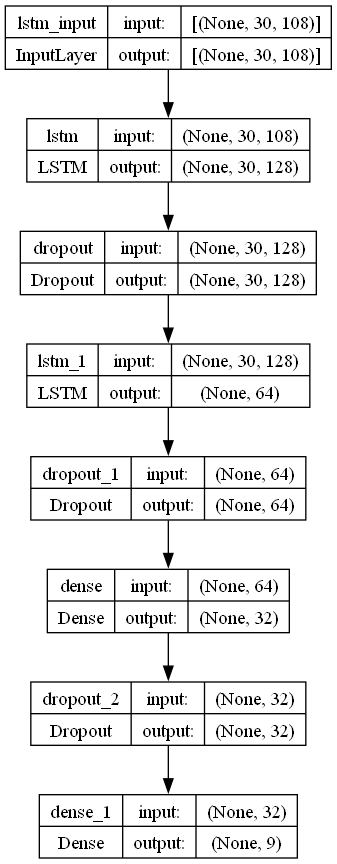
\includegraphics[scale=0.5]{gambar/bab4-uji-model-worst-model.png}

  \caption{Struktur model pertama}
  \label{fig:model1-struktur}
\end{figure}

Berdasarkan dari \emph{training} yang telah dilakukan didapatkan bahwa model menghasilkan akurasi validasi bernilai 0.89 dan akurasi \emph{training} bernilai 0.71. Data ini menunjukkan bahwa model memiliki akurasi yang cukup baik. Untuk nilai \emph{loss training} bernilai cukup tinggi, yaitu bernilai 2.81 dan \emph{loss} validasi bernilai 0.76 yang cukup rendanh jika dibandingkan dengan nilai \emph{loss training}. Nilai dari \emph{loss training} terlihat melonjak di \emph{epoch} terakhir, yaitu pada \emph{epoch} 12. Hal ini selaras dengan penurunan \emph{accuracy} model setelah \emph{epoch} 10. Grafik akurasi dan \emph{loss} dapat dilihat pada gambar \ref{fig:model1-train-acc} dan gambar \ref{fig:model1-train-loss}.

\begin{figure}[H]
  \centering

  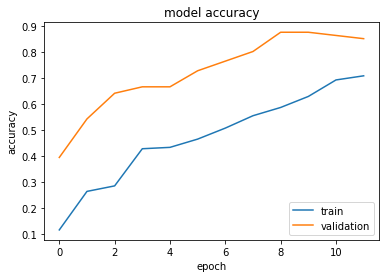
\includegraphics[scale=0.75]{gambar/bab4-uji-model-worst-acc.png}

  \caption{Hasil \emph{accuracy} model pertama}
  \label{fig:model1-train-acc}
\end{figure}

\begin{figure}[H]
  \centering

  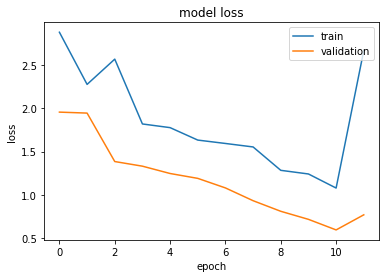
\includegraphics[scale=0.75]{gambar/bab4-uji-model-worst-loss.png}

  \caption{Hasil \emph{loss} model pertama}
  \label{fig:model1-train-loss}
\end{figure}

Kemudian berdasarkan model yang telah dihasilkan, dilakukan pengujian dengan dataset \emph{testing} yang menghasilkan \emph{confusion matrix}. Dapat dilihat pada gambar \ref{fig:model1-cf}, untuk kosakata "maaf", "tolong", "rumah", "delete", dan "translate" menghasilkan prediksi yang tepat untuk keseluruhan dataset \emph{testing} yang diujikan. Namun, kosakata "nama", "saya", "siapa", dan "standby" menghasilkan beberapa prediksi yang tidak sesuai dengan dataset \emph{testing}. Kosakata "nama" menghasilkan 6 prediksi tepat dan 4 prediksi yang kurang tepat (1 dataset \emph{testing} bernilai "siapa" dan 3 dataset \emph{testing} bernilai "rumah"). Kosakata "saya" menghasilkan 10 prediksi tepat dan 2 prediksi yang kurang tepat (dataset \emph{testing} bernilai "translate"). Kosakata "siapa" menghasilkan 3 prediksi tepat dan 5 prediksi yang kurang tepat (2 dataset \emph{testing} bernilai "tolong",  2 dataset \emph{testing} bernilai "saya", dan 1 dataset \emph{testing} bernilai "translate"). Kosakata "standby" menghasilkan 7 prediksi tepat dan 1 prediksi yang kurang tepat (dataset \emph{testing} bernilai "saya"). Adapun berdasarkan hasil \emph{confusion matrix} ini didapat matrix evaluasi berupa \emph{accuracy}, \emph{precision}, \emph{recall}, dan \emph{F1-score} yang dapat dilihat pada tabel \ref{tb:model1stat}. Rata - rata nilai \emph{accuracy} sebesar 0.85, rata - rata nilai \emph{precision} sebesar 0.85, rata - rata nilai \emph{recall} sebesar 0.85, dan rata - rata nilai \emph{F1-score} sebesar 0.83.

\begin{figure}[H]
  \centering

  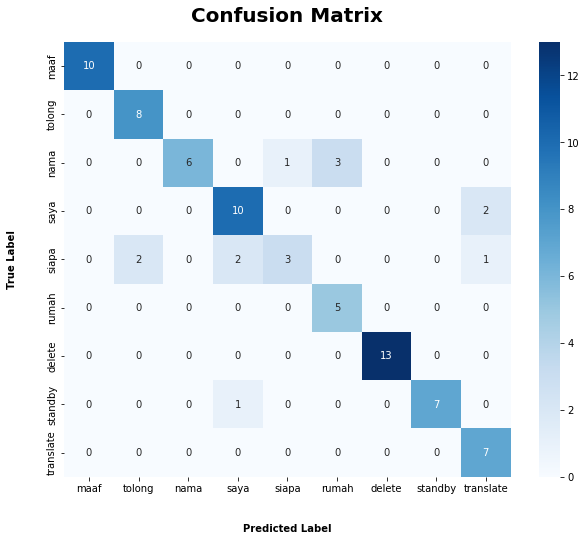
\includegraphics[scale=0.6]{gambar/bab4-uji-model-worst-cf.png}

  \caption{\emph{Confusion} model pertama}
  \label{fig:model1-cf}
\end{figure}

\begin{longtable}{|c|c|c|c|c|}
  \caption{Matrix Evaluasi Model 1}
  \label{tb:model1stat}                                   \\
  \hline
  \rowcolor[HTML]{C0C0C0}
  \textbf{Kosakata} & \textbf{\emph{Accuracy}} & \textbf{\emph{Precision}} & \textbf{\emph{Recall}} & \textbf{\emph{F1-Score}} \\
  \hline
  Maaf              & 1.00                     & 1.00                        & 1.00                   & 1.00                \\
  Tolong            & 1.00                     & 0.80                        & 1.00                   & 0.89                \\
  Nama              & 0.60                     & 1.00                        & 0.60                   & 0.75                \\
  Saya              & 0.83                     & 0.77                        & 0.83                   & 0.80                \\
  Siapa             & 0.37                     & 0.75                        & 0.38                   & 0.50                \\
  Rumah             & 1.00                     & 0.62                        & 1.00                   & 0.77                \\
  Delete            & 1.00                     & 1.00                        & 1.00                   & 1.00                \\
  Standby           & 0.87                     & 1.00                        & 0.88                   & 0.93                \\
  Translate         & 1.00                     & 0.70                        & 1.00                   & 0.82                \\
  \hline
\end{longtable}

\subsection{Model Kedua}
\label{sec:analisismodel2}

Model kedua diawali dengan \emph{layer} \textit{TimeDistributed} yang di dalamnya terdapat \emph{layer} \textit{Dense} dengan fungsi aktivasi '\textit{tanh}' dan unit aktivasi bernilai 128. Kemudian dilanjutkan dengan 1 buah \emph{layer} LSTM yang menggunakan fungsi aktivasi \emph{tanh} dan dengan unit aktivasi bernilai 64. \emph{Layer} LSTM akan diikuti dengan \emph{layer} Dropout bernilai 0.5 untuk mencegah nilai \emph{weight} yang terlalu tinggi. Setelah serangkaian \emph{layer} LSTM, diikuti dengan \emph{layer} Dense dengan fungsi aktivasi \emph{relu} dan dengan unit aktivasi bernilai 32. Struktur lengkap dari model ini dapat dilihat pada \ref{fig:model2-struktur}.

\begin{figure}[H]
  \centering

  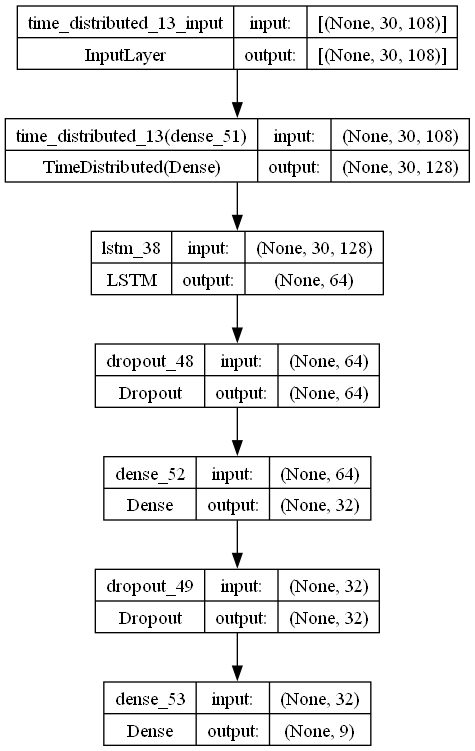
\includegraphics[scale=0.6]{gambar/bab4-uji-model-second-model.png}

  \caption{Struktur model kedua}
  \label{fig:model2-struktur}
\end{figure}

Berdasarkan dari \emph{training} yang telah dilakukan didapatkan bahwa model menghasilkan akurasi \emph{training} bernilai 0.96 dan akurasi validasi bernilai 0.93. Data ini menunjukkan bahwa model memiliki akurasi yang baik. Terdapat penurunan pada akurasi validasi pada \emph{epoch} terakhir, tetapi kebalikannya untuk akurasi \emph{training} mengalami kenaikan melebihi akurasi validasi. Untuk nilai \emph{loss training} bernilai 0.32 dan \emph{loss} validasi bernilai 0.25 yang cukup rendah jika dibandingkan dengan nilai \emph{loss training}. Data ini menunjukkan bahwa model memiliki \emph{error} prediksi yang kecil. Grafik akurasi dan \emph{loss} dapat dilihat pada gambar \ref{fig:model2-train-acc} dan gambar \ref{fig:model2-train-loss}.

\begin{figure}[H]
  \centering

  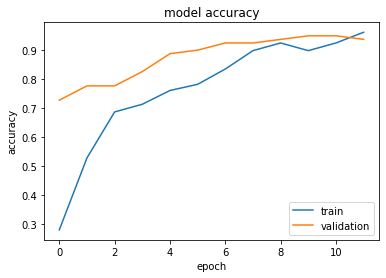
\includegraphics[scale=0.75]{gambar/bab4-uji-model-second-acc.png}

  \caption{Hasil \emph{accuracy} model kedua}
  \label{fig:model2-train-acc}
\end{figure}

\begin{figure}[H]
  \centering

  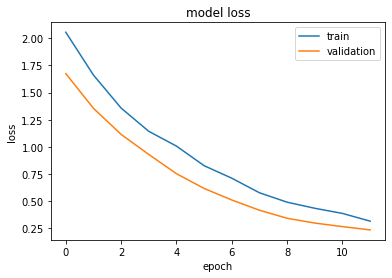
\includegraphics[scale=0.75]{gambar/bab4-uji-model-second-loss.png}

  \caption{Hasil \emph{loss} model kedua}
  \label{fig:model2-train-loss}
\end{figure}


Kemudian berdasarkan model yang telah dihasilkan, dilakukan pengujian dengan dataset \emph{testing} yang menghasilkan \emph{confusion matrix}. Dapat dilihat pada gambar \ref{fig:model2-cf}, untuk kosakata "tolong", "nama", "rumah", "delete", dan "translate" menghasilkan prediksi yang tepat untuk keseluruhan dataset \emph{testing} yang diujikan. Namun, kosakata "saya", "siapa", dan "standby" menghasilkan beberapa prediksi yang tidak sesuai dengan dataset \emph{testing}. Kosakata "maaf" menghasilkan 10 prediksi tepat dan 1 prediksi yang kurang tepat (dataset \emph{testing} bernilai "standb\\y"). Kosakata "saya" menghasilkan 11 prediksi tepat dan 2 prediksi yang kurang tepat (dataset \emph{testing} bernilai "siapa"). Kosakata "siapa" menghasilkan 5 prediksi tepat dan 1 prediksi yang kurang tepat (dataset \emph{testing} bernilai "saya"). Kosakata "standby" menghasilkan 7 prediksi tepat dan 1 prediksi yang kurang tepat (dataset \emph{testing} bernilai "siapa"). Dapat dilihat bahwa terdapat peningkatan performa dari model pertama dengan model kedua. Kosakata yang berhasil diprediksi sesuai dengan dataset \emph{testing} yang digunakan lebih banyak dibandingkan dengan model sebelumnya, yaitu 5 kosakata. Peningkatan ini disebabkan karena perubahan struktur dari model dengan adanya penggunaan \emph{layer Time Distributed} yang di dalamnya diisi dengan \emph{layer} Dense di lapisan awal model. Pengurangan pengunaan 1 \emph{layer} LSTM dapat dengan menggunakan fungsi aktivasi \emph{tanh}. Adapun berdasarkan \emph{confusion matrix} ini didapat matrix evaluasi berupa \emph{accuracy}, \emph{precision}, \emph{recall}, dan \emph{F1-score} yang dapat dilihat pada tabel \ref{tb:model2stat}. Rata - rata nilai \emph{accuracy} sebesar 0.93, nilai \emph{precision} sebesar 0.95, rata - rata nilai \emph{recall} sebesar 0.94, dan rata - rata nilai \emph{F1-score} sebesar 0.94. Dapat dilihat berdasarkan matrix evaluasi ini, terdapat peningkatan performa pada model kedua jika dibandingkan dengan model pertama. 

\begin{figure}[H]
  \centering

  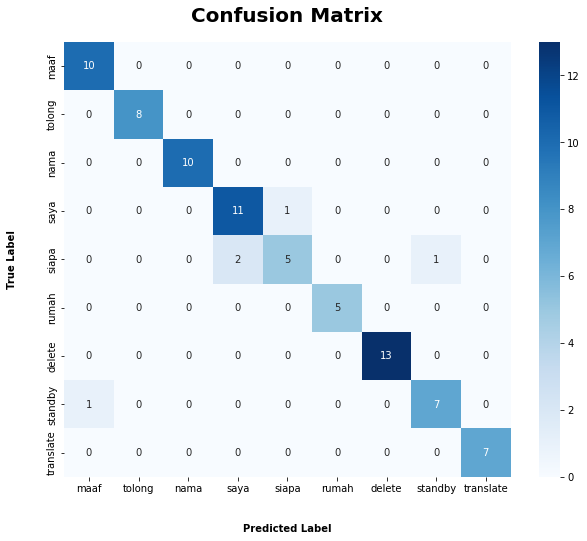
\includegraphics[scale=0.6]{gambar/bab4-uji-model-second-cf.png}

  \caption{\emph{Confusion} model kedua}
  \label{fig:model2-cf}
\end{figure}

\begin{longtable}{|c|c|c|c|c|}
  \caption{Matrix Evaluasi Model 2}
  \label{tb:model2stat}                                   \\
  \hline
  \rowcolor[HTML]{C0C0C0}
  \textbf{Kosakata} & \textbf{\emph{Accuracy}} & \textbf{\emph{Precision}} & \textbf{\emph{Recall}} & \textbf{\emph{F1-Score}} \\
  \hline
  Maaf              & 1.00                        & 0.91                        & 1.00                   & 0.95                \\
  Tolong            & 1.00                        & 1.00                        & 1.00                   & 1.00                \\
  Nama              & 1.00                        & 1.00                        & 1.00                   & 1.00                \\
  Saya              & 0.91                        & 0.85                        & 0.92                   & 0.88                \\
  Siapa             & 0.62                        & 0.93                        & 0.62                   & 0.71                \\
  Rumah             & 1.00                        & 1.00                        & 1.00                   & 1.00                \\
  Delete            & 1.00                        & 1.00                        & 1.00                   & 1.00                \\
  Standby           & 0.87                        & 0.88                        & 0.88                   & 0.88                \\
  Translate         & 1.00                        & 1.00                        & 1.00                   & 1.00                \\
  \hline
\end{longtable}

\subsection{Model Ketiga}
\label{sec:analisismodel3}

Model ketiga merupakan gabungan dari struktur antara model 1 dan model 2. Model ini diawali dengan layer pertama berupa \emph{layer} \textit{TimeDistributed} yang di dalamnya terdapat \emph{layer} \textit{Dense} dengan fungsi aktivasi '\textit{tanh}' dan unit aktivasi bernilai 128. Selanjutnya diikuti dengan 2 buah \emph{layer} LSTM. \emph{Layer} LSTM pertama menggunakan fungsi aktivasi \emph{tanh} dengan unit aktivasi bernilai 128 dan \emph{Layer} LSTM kedua menggunakan fungsi aktivasi \emph{tanh} dengan unit aktivasi bernilai 64. Kedua \emph{layer} LSTM ini diikuti dengan \emph{layer} Dropout bernilai 0.5 untuk mencegah nilai \emph{weight} yang terlalu tinggi. Dilanjutkan dengan \emph{layer} Dense dengan fungsi aktivasi \emph{relu} dan unit aktivasi bernilai 32. Struktur lengkap dari model ini dapat dilihat pada gambar \ref{fig:model3-struktur}

\begin{figure}[H]
  \centering

  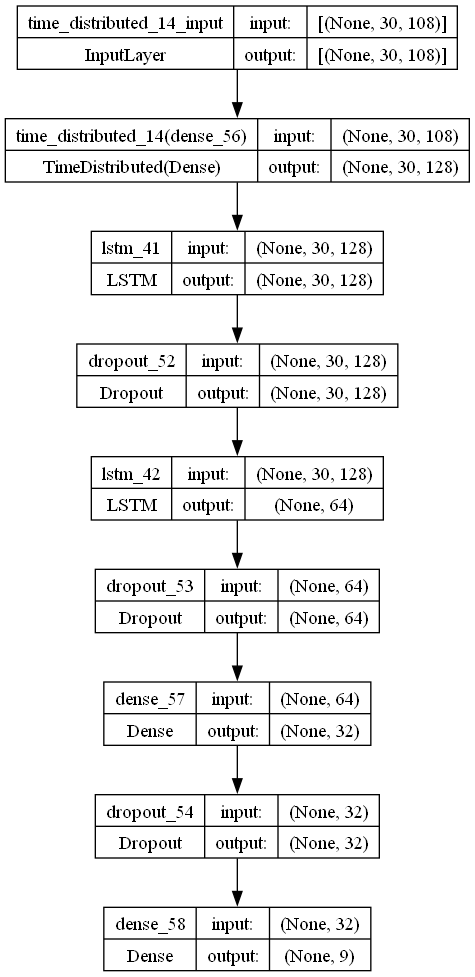
\includegraphics[scale=0.5]{gambar/bab4-uji-model-best-model.png}

  \caption{Struktur model ketiga}
  \label{fig:model3-struktur}
\end{figure}

Berdasarkan dari \emph{training} yang telah dilakukan didapatkan bahwa model menghasilkan akurasi \emph{training} bernilai 0.94 dan akurasi validasi bernilai 1.00. Data ini menunjukkan bahwa model memiliki akurasi yang sangat baik. Untuk nilai \emph{loss training} bernilai 0.3 dan \emph{loss} validasi bernilai 0.16 yang rendah jika dibandingkan dengan nilai \emph{loss training}. Data ini menunjukkan bahwa model memiliki \emph{error} prediksi yang kecil. Hasil dari \emph{training} model ini menunjukkan bahwa model telah dapat mempelajari dataset dengan baik. Ketika dilakukan pengujian dengan menggunakan data validasi, dapat dilihat bahwa model memiliki akurasi yang lebih tinggi dan tingkat \emph{loss} yang lebih rendah dibandingkan dengan pengujian yang menggunakan data \emph{training} itu sendiri. Grafik akurasi dan \emph{loss} dapat dilihat pada gambar \ref{fig:model3-train-acc} dan gambar \ref{fig:model3-train-loss}.

\begin{figure}[H]
  \centering

  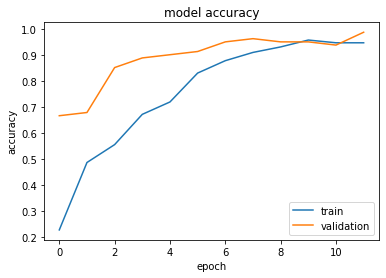
\includegraphics[scale=0.75]{gambar/bab4-uji-model-best-acc.png}

  \caption{Hasil \emph{accuracy} model ketiga}
  \label{fig:model3-train-acc}
\end{figure}

\begin{figure}[H]
  \centering

  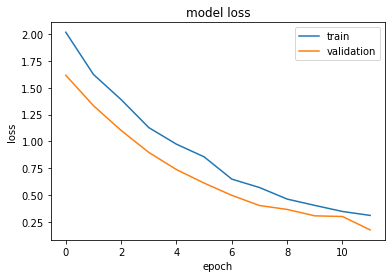
\includegraphics[scale=0.75]{gambar/bab4-uji-model-best-loss.png}

  \caption{Hasil \emph{loss} model ketiga}
  \label{fig:model3-train-loss}
\end{figure}


Kemudian berdasarkan model yang telah dihasilkan, dilakukan pengujian dengan dataset \emph{testing} yang menghasilkan \emph{confusion matrix}. Dapat dilihat pada gambar \ref{fig:model3-cf}, untuk kosakata "maaf", "tolong", "nama", "saya",  menghasilkan prediksi yang tepat untuk keseluruhan dataset \emph{testing} yang diujikan. Namun, pada kosakata "siapa" menghasilkan beberapa prediksi yang tidak sesuai dengan dataset \emph{testing}. Kosakata "siapa" menghasilkan 7 prediksi tepat dan 1 prediksi yang kurang tepat (dataset \emph{testing} bernilai "saya"). Dapat dilihat bahwa terdapat peningkatan performa dari model ketiga dibandingkan dengan model pertama dan kedua. Peningkatan ini disebabkan karena perubahan struktur dari model dengan penggunaan \emph{layer Time Distributed} yang didalamnya diisi dengan \emph{layer} Dense di lapisan awal model. Kemudian dilanjutkan dengan 2 buah \emph{layer} LSTM yang menggunakan fungsi aktivasi \emph{tanh} Adapun berdasarkan \emph{confusion matrix} ini didapat matrix evaluasi berupa \emph{accuracy}, \emph{precision}, \emph{recall}, dan \emph{F1-score} yang dapat dilihat pada tabel \ref{tb:model3stat}. Rata - rata nilai \emph{accuracy} sebesar 0.99, rata - rata nilai \emph{precision} sebesar 0.99 rata - rata nilai \emph{recall} sebesar 0.98, dan rata - rata nilai \emph{F1-score} sebesar 0.99. Dapat dilihat berdasarkan matrix evaluasi ini, terdapat peningkatan performa pada model ketiga jika dibandingkan dengan model pertama dan kedua.

\begin{figure}[H]
  \centering

  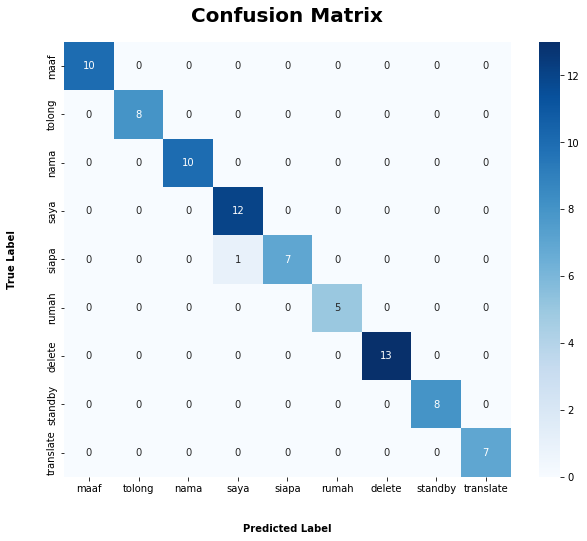
\includegraphics[scale=0.6]{gambar/bab4-uji-model-best-cf.png}

  \caption{\emph{Confusion} model pertama}
  \label{fig:model3-cf}
\end{figure}

\newpage
\begin{longtable}{|c|c|c|c|c|c|}
  \caption{Matrix Evaluasi Model 3}
  \label{tb:model3stat}                                   \\
  \hline
  \rowcolor[HTML]{C0C0C0}
  \textbf{Kosakata} & \textbf{\emph{Accuracy}} & \textbf{\emph{Precision}} & \textbf{\emph{Recall}} & \textbf{\emph{F1-Score}} \\
  \hline
  Maaf              & 1.00                       & 1.00                        & 1.00                   & 1.00                \\
  Tolong            & 1.00                       & 1.00                        & 1.00                   & 1.00                \\
  Nama              & 1.00                       & 1.00                        & 1.00                   & 1.00                \\
  Saya              & 1.00                       & 0.92                        & 1.00                   & 0.96                \\
  Siapa             & 0.87                       & 1.00                        & 0.82                   & 0.93                \\
  Rumah             & 1.00                       & 1.00                        & 1.00                   & 1.00                \\
  Delete            & 1.00                       & 1.00                        & 1.00                   & 1.00                \\
  Standby           & 1.00                       & 1.00                        & 1.00                   & 1.00                \\
  Translate         & 1.00                       & 1.00                        & 1.00                   & 1.00                \\
  \hline
\end{longtable}

\subsection{Rangkuman Pengujian Bentuk Model}
\label{sec:analisismodelseluruh}

\begin{longtable}{|c|c|c|c|c|}
  \caption{Rangkuman Pengujian Bentuk Model}
  \label{tb:evaluasiModel}                                   \\
  \hline
  \rowcolor[HTML]{C0C0C0}
  \textbf{Model} & \emph{\textbf{Avg. Accuracy}} & \emph{\textbf{Avg. Precision}} & \emph{\textbf{Avg. Recall}} & \emph{\textbf{Avg. F1-Score}} \\
  \hline
  Model 1 & 0.85 & 0.85 & 0.85 & 0.83 \\
  Model 2 & 0.93 & 0.95 & 0.94 & 0.94 \\
  Model 3 & 0.99 & 0.99 & 0.98 & 0.99 \\
  \hline
\end{longtable}

Secara keseluruhan, berdasarkan tabel \ref{tb:evaluasiModel} bahwa seiring denagn peningkatan kompleksitas dari suatu model selaras dengan peningkatan performa dari model itu sendiri. Hal ini dapat ditunjukkan dengan peningkatan akurasi dari model 1, yaitu 0.85 atau 85\% menjadi pada model 3, yaitu 0.99 atau 99\%. Nilai \emph{average precision}, {average recall},dan \emph{average F1-Score} juga meningkat seiring dengan peningkatan stuktur dari model. Penggunaan \emph{layer TimeDistributed} dan diikuti 2 \emph{layer} LSTM menghasilkan model dengan performa terbaik.

\section{Pengujian Kondisi Cahaya}
\label{sec:analisiscahaya}

Pada pengujian kondisi cahaya ini dilakukan untuk memahami bagaimana performa model dalam kondisi intensitas cahaya  yang berbeda - beda. Adapun intensitas cahaya yang akan digunakan pada pengujian ini adalah 35 lux (kondisi ruangan gelap), 80 lux (kondisi ruangan remang - remang), dan 125 lux (kondisi ruangan terang). Variasi intensitas cahaya ini dipilih karena merupakan intensitas cahaya yang umum ditemukan pada ruangan tertutup. Kondisi ruangan dengan intensitas cahaya masing - masing dapat dilihat pada tabel \ref{tb:kondisicahaya}. Pengambilan nilai intensitas cahaya ini dilakukan dengan menggunakan \emph{lux meter} yang telah dikalibrasi untuk memastikan ketelitian hasil pengukuran.

Model penerjemah bahasa Indonesia (BISINDO) yang akan digunakan pada pengujian ini adalah model pada bagian \ref{sec:analisismodel3} karena merupakan model yang menghasilkan klasifikasi yang terbaik jika dibandingkan dengan model lainnya. Untuk setiap intensitas cahaya akan dilakukan pengujian sebanyak tiga kali dengan jarak terhadap kamera sebesar 300 cm. Pada setiap pengujian akan dicari hasil klasifikasi model, waktu yang dibutuhkan model untuk menghasilkan klasifikasi bahasa isyarat berdasarkan data koordinat yang diberikan(\emph{processing time}), dan waktu total yang dibutuhkan dalam menghasilkan klasifikasi bahasa isyarat (\emph{complete time}).  

\newpage
\begin{longtable}{|c|c|}
  \caption{Variasi Kondisi Cahaya}
  \label{tb:kondisicahaya}                                   \\
  \hline
  \rowcolor[HTML]{C0C0C0}
  \textbf{Intensitas Cahaya} & \textbf{Gambar Kondisi}  \\
  \hline
  35 lux            &  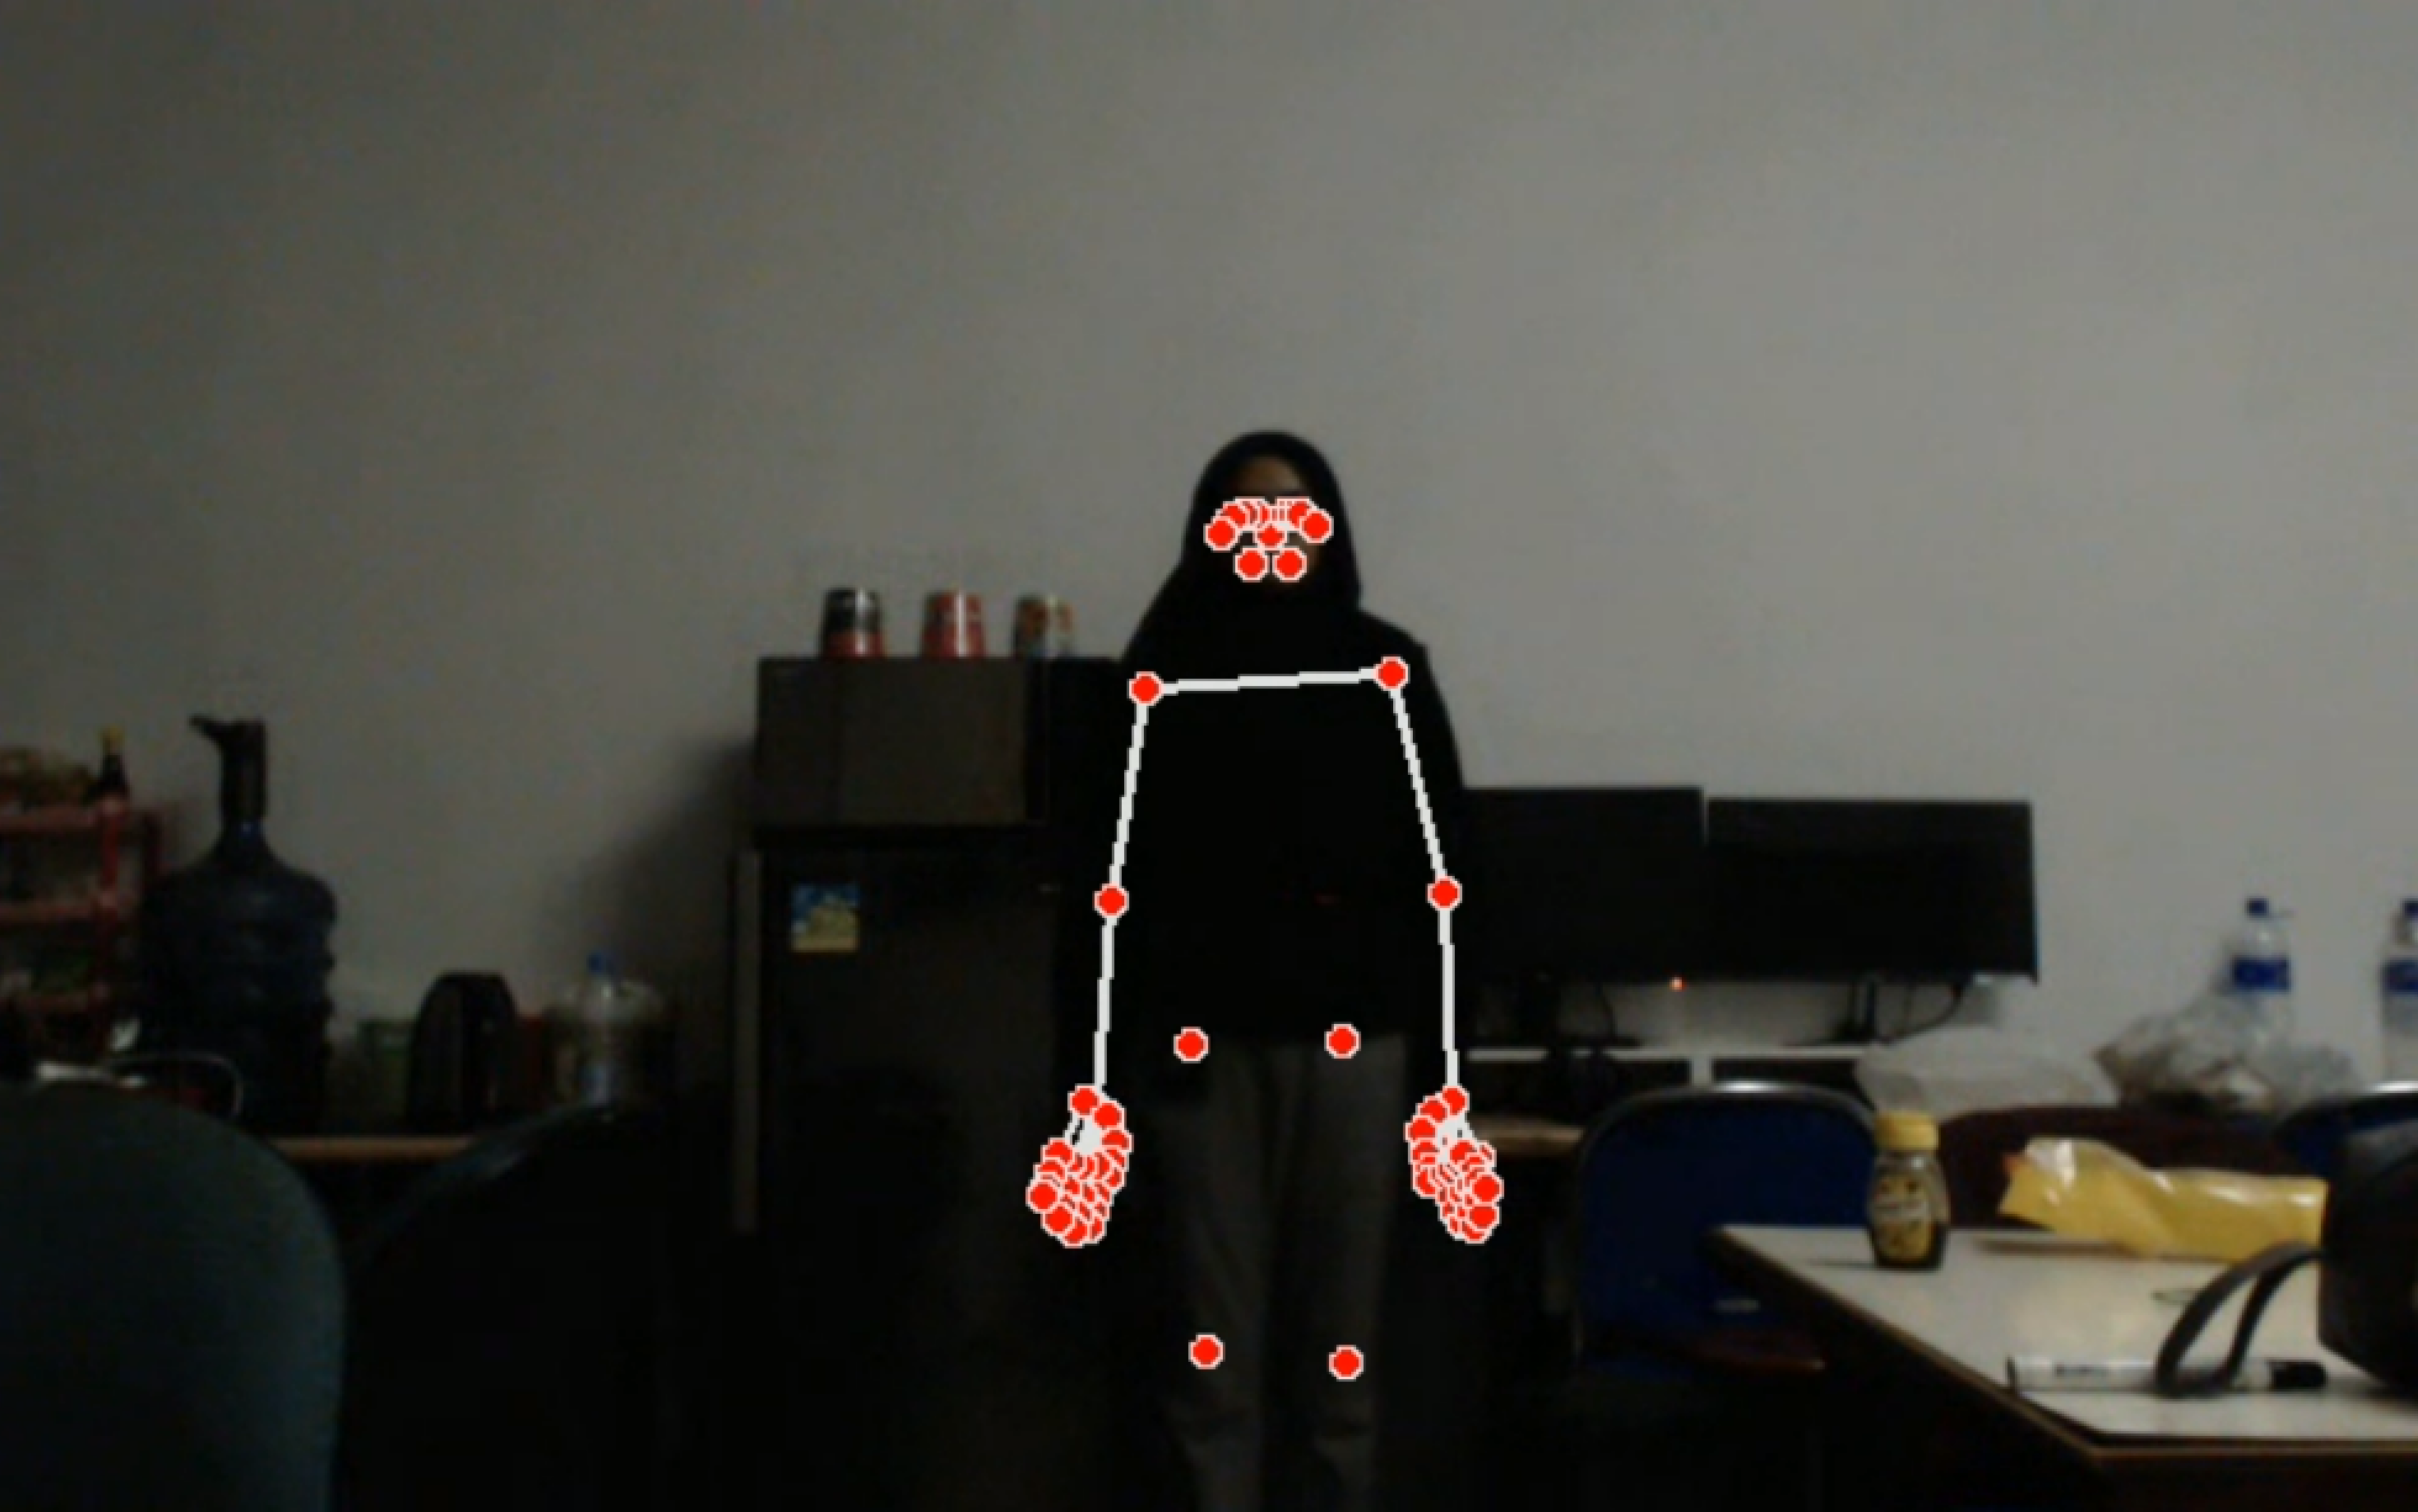
\includegraphics[scale=0.3]{gambar/bab4-gelap.png}                \\
  \hline
  80 lux            & 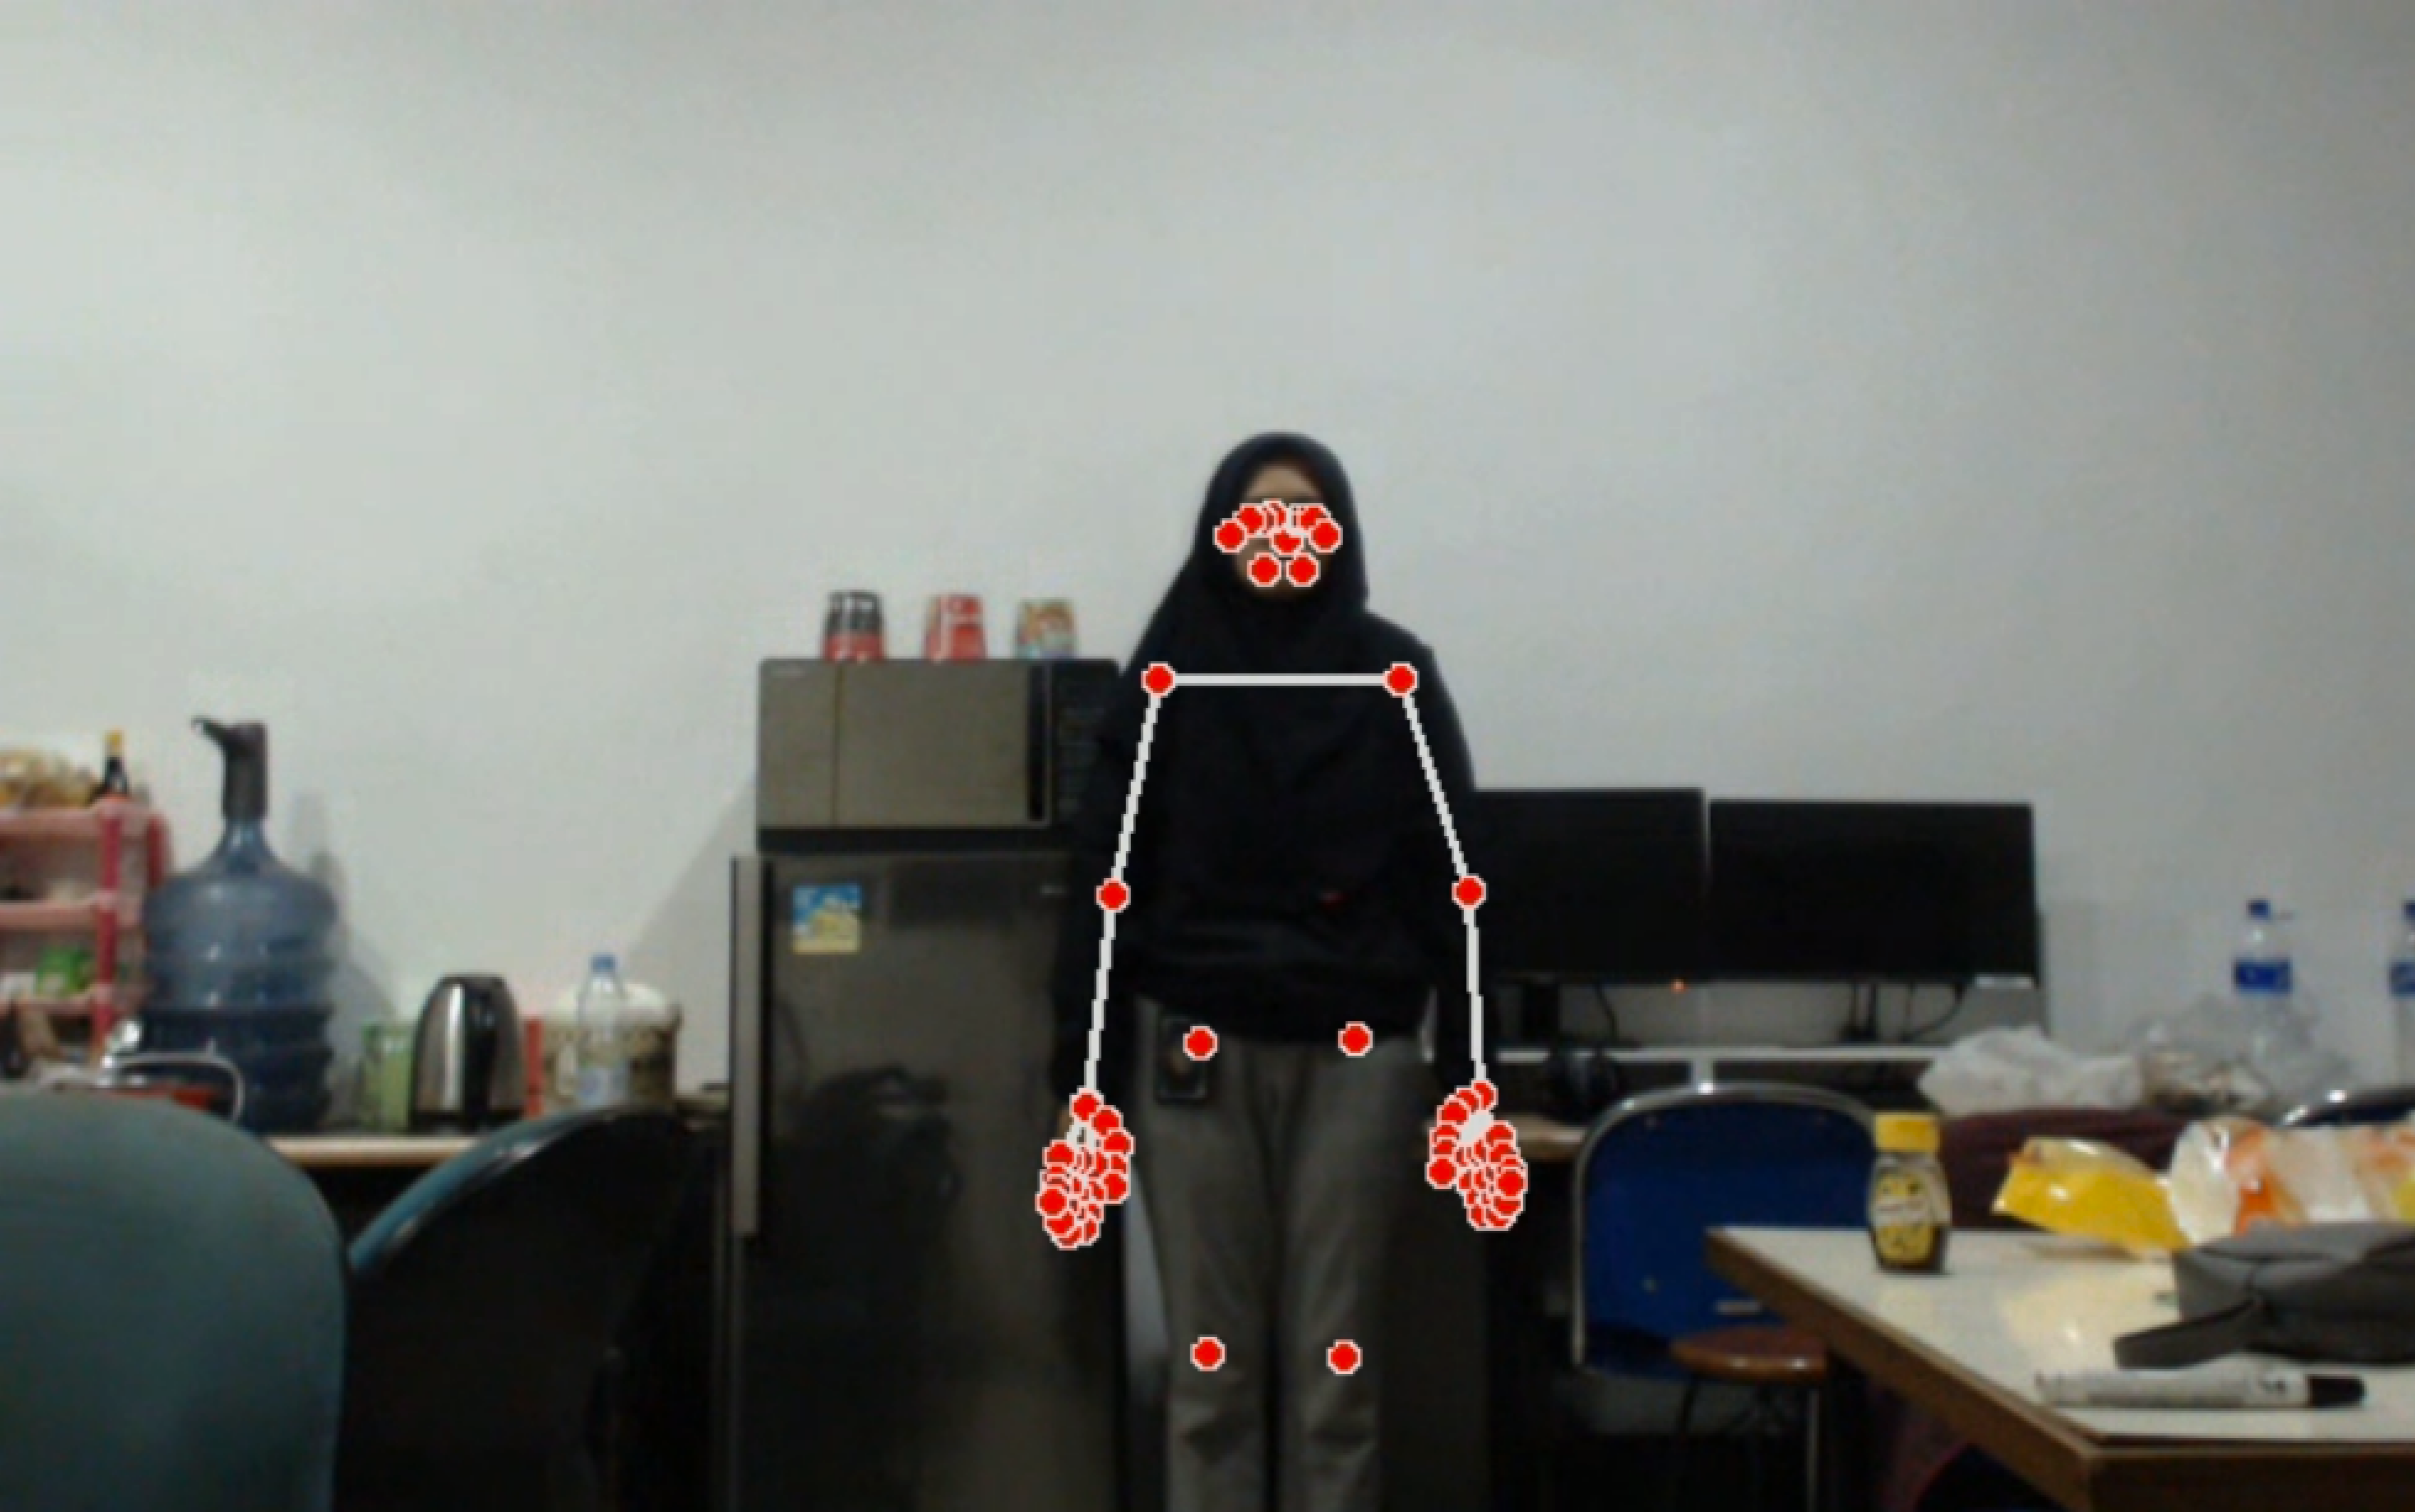
\includegraphics[scale=0.3]{gambar/bab4-remang.png}                 \\
  \hline
  125 lux            & 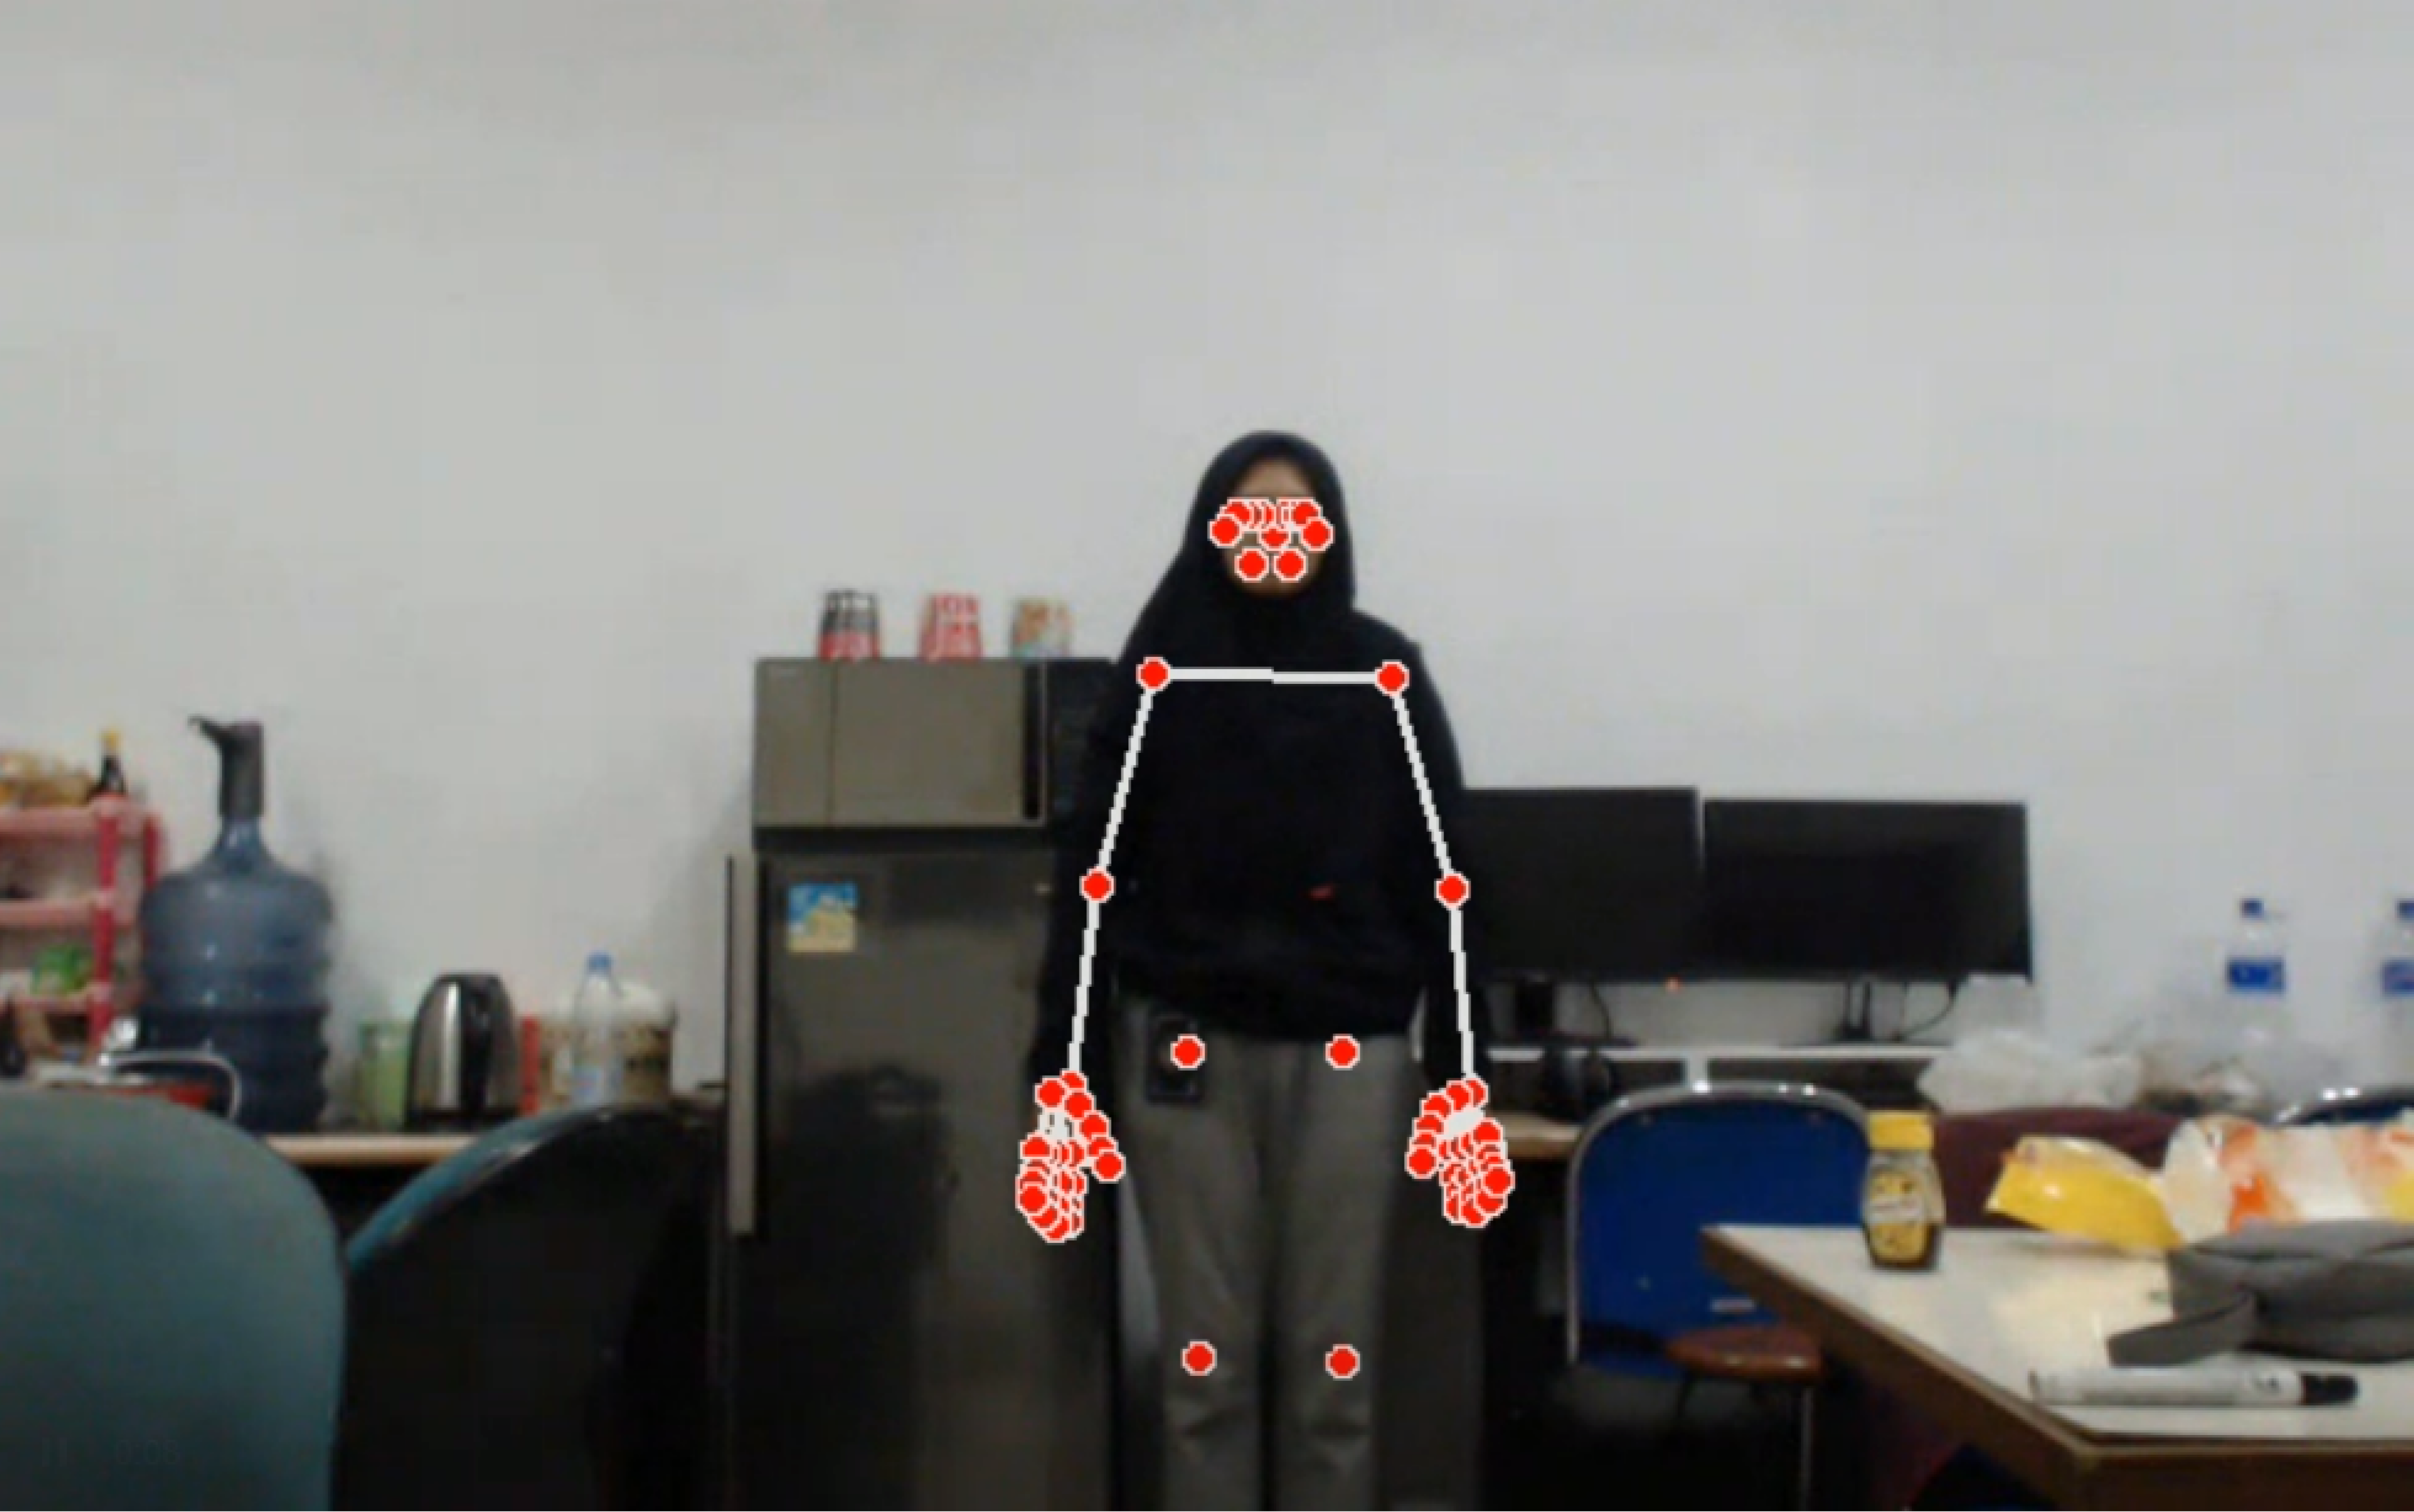
\includegraphics[scale=0.3]{gambar/bab4-terang.png}                 \\
  \hline
\end{longtable}

\newpage
\subsection{Pengujian Model di Kondisi Cahaya 35 lux}
\label{sec:analisiscahaya1}

\begin{longtable}{|c|c|c|c|}
  \caption{Pengujian Pertama Model di Kondisi Cahaya 35 lux}
  \label{tb:prediksigelap1}                                   \\
  \hline
  \rowcolor[HTML]{C0C0C0}
  \textbf{Kosakata} & \textbf{Klasifikasi Model} & \textbf{\emph{Processing Time}} & \textbf{\emph{Complete Time}}\\
  \hline
  Maaf              & Maaf                          & 0.09208822250366211 detik                           & 2.8735828399658203 detik                                  \\
  Tolong            & Tolong                        & 0.09197822450361212 detik                           & 2.9096102714538574 detik                                  \\
  Nama              & Nama                          & 0.08932256698608398 detik                           & 3.3274698257446294 detik                                  \\
  Saya              & Saya                          & 0.09866833686828613 detik                           & 2.8822731971740723 detik                                  \\
  Siapa             & Siapa                         & 0.08973073959350586 detik                           & 2.8529834747314453 detik                                  \\
  Rumah             & \textcolor{red}{Delete}       & 0.09612202644348145 detik                           & 2.8643417358398438 detik                                  \\
  Delete            & Delete                        & 0.09255480766296387 detik                           & 2.824845314025879 detik                                 \\
  Standby           & Standby                       & 0.09247112274169922 detik                           & 2.8762435913085938 detik                                  \\
  Translate         & Translate                     & 0.09525346755981445 detik                           & 2.9262471199035645 detik                                  \\
  \hline
\end{longtable}

\begin{longtable}{|c|c|c|c|}
  \caption{Pengujian Kedua Model di Kondisi Cahaya 35 lux}
  \label{tb:prediksigelap2}                                   \\
  \hline
  \rowcolor[HTML]{C0C0C0}
  \textbf{Kosakata} & \textbf{Klasifikasi Model} & \textbf{\emph{Processing Time}} & \textbf{\emph{Complete Time}} \\
  \hline
  Maaf              & Maaf                            & 0.10043215751647949 detik                           & 3.328549861907959 detik                                 \\
  Tolong            & Tolong                          & 0.0972287654876709 detik                            & 3.3190798759460445 detik                                  \\
  Nama              & \textcolor{red}{Standby}        & 0.08973073959350586 detik                           & 2.914302349090576 detik                                 \\
  Saya              & Saya                            & 0.1007227897644043 detik                            & 2.789583206176758 detik                                 \\
  Siapa              & Siapa                          & 0.08973073959350586 detik                           & 3.4017491340637203 detik                                  \\
  Rumah             & Rumah                           & 0.10046267509460449 detik                           & 2.94283390045166 detik                                \\
  Delete            & Delete                          & 0.09255480766296387 detik                           & 2.9163265228271484 detik                                  \\
  Standby           & Standby                         & 0.09181642532348633 detik                           & 2.8268051147460938 detik                                  \\
  Translate         & Translate                       & 0.08920478820800781 detik                           & 3.3912491798400874 detik                                  \\
  \hline
\end{longtable}

\begin{longtable}{|c|c|c|c|}
  \caption{Pengujian Ketiga Model di Kondisi Cahaya 35 lux}
  \label{tb:prediksigelap3}                                   \\
  \hline
  \rowcolor[HTML]{C0C0C0}
  \textbf{Kosakata} & \textbf{Klasifikasi Model} & \textbf{\emph{Processing Time}} & \textbf{\emph{Complete Time}}\\
  \hline
  Maaf              & Maaf                          & 0.09208822250366211 detik                           & 2.9158973693847656 detik                                  \\
  Tolong            & Tolong                        & 0.0972287654876709 detik                            & 3.0014920234680176 detik                                  \\
  Nama              & Nama                          & 0.09724950790405273 detik                           & 2.8235292434692383 detik                                  \\
  Saya              & Saya                          & 0.08916234970092773 detik                           & 2.9606938362121578 detik                                  \\
  Siapa             & Siapa                         & 0.08973073959350586 detik                           & 2.8408455848693848 detik                                  \\
  Rumah             & \textcolor{red}{Delete}       & 0.10066267509460449 detik                           & 3.36672306060791 detik                                \\
  Delete            & Delete                        & 0.09255480766296387 detik                           & 3.4308242797851562 detik                                  \\
  Standby           & Standby                       & 0.09866833686828613 detik                           & 3.3450722694396973 detik                                  \\
  Translate         & Translate                     & 0.08920478820800781 detik                           & 2.830524444580078 detik                                 \\
  \hline
\end{longtable}

Berdasarkan tiga pengujian yang telah dilakukan, didapatkan bahwa hampir keseluruhan klasifikasi model yang sesuai dengan \emph{class} kosakata. Namun, terdapat beberapa kesalahan model dalam melakukan klasifikasi. Dapat dilihat pada tabel \ref{tb:prediksigelap1} untuk kosakata "Rumah" diklasifikasikan sebagai "Delete". Kesalahan ini juga terjadi pada tabel \ref{tb:prediksigelap3}. Kemiripan antara gerakan untuk isyarat kosakata "Rumah" dan "Delete", serta kamera yang kesulitan menangkap sepenuhnya pose yang baik menjadi penyebab adanya kesalahan klasifikasi ini. Pada tabel \ref{tb:prediksigelap2}, untuk isyarat kosakata "Nama" diklasifikasikan sebagai "Standby". Kesalahan klasifikasi ini juga disebabkan oleh Mediapipe yang tidak sepenuhnya menangkap pose yang sesuai dengan kosakata "Nama". Pada pengujian ini,  model dapat melakukan klasifikasi yang baik meskipun pengguna berada di dalam kondisi ruangan yang terbilang gelap. Berdasakan data pada tabel \ref{tb:prediksigelap1}, tabel \ref{tb:prediksigelap2}, tabel \ref{tb:prediksigelap3} menunjukkan bahwa secara keseluruhan model memiliki akurasi klasifikasi sebesar 89.9\%. 

Apabila dilihat berdasarkan waktu pemrosesan, rata - rata waktu yang dibutuhkan model untuk menghasilkan klasifikasi bahasa isyarat (\emph{processing time}) adalah 0.093 detik dan rata - rata waktu yang dibutuhkan dalam menghasilkan klasifikasi bahasa isyarat (\emph{complete time}) adalah 3.025 detik. Pada proses pengujian yang dilakukan secara \emph{real time} ini, model memerlukan waktu yang terbilang cepat dalam memproses serangkaian data koordinat yang diberikan. Program penerjemah juga telah mampu menyelesaikan proses klasifikasi dengan cepat. Hal ini menunjukkan bahwa pada kondisi ruangan dengan intensitas cahaya yang cukup gelap, tidak berpengaruh secara signifikan terhadap \emph{processing time} dan \emph{complete time}.

Pada pengujian di intensitas cahaya 35 lux, didapat bahwa pengguna tidak dapat melakukan gerakan bahasa isyarat secara cepat. Hal ini disebabkan oleh kondisi ruangan yang gelap ini mempengaruhi kinerja kemmapuan kamera dalam menangkap tiap \emph{frame}. Namun, kemampuan \emph{framework} Mediapipe untuk mendeteksi pose pengguna dan melakukan ekstraksi koordinat berdasarkan \emph{landmark} yang ada masih dapat berjalan dengan baik pada kondisi ruangan dengan intensitas cahaya yang kurang baik. Hal ini membantu proses klasifikasi model karena data koordinat yang diproses untuk menghasilkan klasifikasi bahasa isyarat tetap dapat dieksraksi dengan tepat dan tidak memiliki banyak error atau data koordinat kosong (bernilai 0). 

\subsection{Pengujian Model di Kondisi Cahaya 80 lux}
\label{sec:analisiscahaya2}

\begin{longtable}{|c|c|c|c|}
  \caption{Pengujian Pertama Model di Kondisi Cahaya 80 lux}
  \label{tb:prediksiremang1}                                   \\
  \hline
  \rowcolor[HTML]{C0C0C0}
  \textbf{Kosakata} & \textbf{Klasifikasi Model} & \textbf{\emph{Processing Time}} & \textbf{\emph{Complete Time}}\\
  \hline
  Maaf              & Maaf                         & 0.09171247482299805 detik                           & 2.749907970428467 detik                                  \\
  Tolong            & Tolong                       & 0.09063005447387695 detik                           & 3.3760499954223637 detik                                   \\
  Nama              & Nama                         & 0.09208822250366211 detik                           & 2.930173873901367 detik                                  \\
  Saya              & Saya                         & 0.09037542343139648 detik                           & 2.723050117492676 detik                                  \\
  Siapa             & Siapa                        & 0.09206461906433105 detik                           & 2.848784923553467 detik                                  \\
  Rumah             & Rumah                        & 0.09352707862854004 detik                           & 2.8643417358398438 detik                                   \\
  Delete            & Delete                       & 0.0890190601348877 detik                            & 2.871215343475342 detik                                  \\
  Standby           & Standby                      & 0.08996152877807617 detik                           & 3.3450722694396973 detik                                   \\
  Translate         & Translate                    & 0.08868694305419922 detik                           & 3.3266687393188477 detik                                   \\
  \hline
\end{longtable}

\newpage
\begin{longtable}{|c|c|c|c|}
  \caption{Pengujian Kedua Model di Kondisi Cahaya 80 lux}
  \label{tb:prediksiremang2}                                   \\
  \hline
  \rowcolor[HTML]{C0C0C0}
  \textbf{Kosakata} & \textbf{Klasifikasi Model} & \textbf{\emph{Processing Time}} & \textbf{\emph{Complete Time}}\\
  \hline
  Maaf              & Maaf                        & 0.09696221351623535 detik                           & 3.2127857208251953 detik                                 \\
  Tolong            & Tolong                      & 0.09327077865600586 detik                           & 2.8273916244506836 detik                                 \\
  Nama              & Nama                        & 0.09208822250366211 detik                           & 2.7649283409118652 detik                                 \\
  Saya              & Saya                        & 0.08996152877807617 detik                           & 3.50247859954834 detik                               \\
  Siapa             & Siapa                       & 0.08884954452514648 detik                           & 2.910640239715576 detik                                \\
  Rumah             & Rumah                       & 0.09037542343139648 detik                           & 2.895984649658203 detik                                \\
  Delete            & Delete                      & 0.0916590690612793 detik                            & 2.876894474029541 detik                                \\
  Standby           & Standby                     & 0.08996152877807617 detik                           & 2.8268051147460938 detik                                 \\
  Translate         & Translate                   & 0.09454655647277832 detik                           & 2.887272834777832 detik                                \\
  \hline
\end{longtable}

\begin{longtable}{|c|c|c|c|}
  \caption{Pengujian Ketiga Model di Kondisi Cahaya 80 lux}
  \label{tb:prediksiremang3}                                   \\
  \hline
  \rowcolor[HTML]{C0C0C0}
  \textbf{Kosakata} & \textbf{Klasifikasi Model} & \textbf{\emph{Processing Time}} & \textbf{\emph{Complete Time}}\\
  \hline
  Maaf              & Maaf                          & 0.08908700942993164 detik                          & 2.8675103187561035 detik                                  \\
  Tolong            & Tolong                        & 0.09565138816833496 detik                          & 2.890141010284424 detik                                 \\
  Nama              & Nama                          & 0.09208822250366211 detik                          & 3.3304882049560547 detik                                  \\
  Saya              & Saya                          & 0.08996152877807617 detik                          & 2.884190082550049 detik                                 \\
  Siapa             & Siapa                         & 0.08884954452514648 detik                          & 2.8408455848693848 detik                                  \\
  Rumah             & \textcolor{red}{Delete}       & 0.08767223358154297 detik                          & 3.3569884300231934 detik                                  \\
  Delete            & Delete                        & 0.0912930965423584 detik                           & 2.8562521934509277 detik                                  \\
  Standby           & Standby                       & 0.08996152877807617 detik                          & 2.8762435913085938 detik                                  \\
  Translate         & Translate                     & 0.09907031059265137 detik                          & 2.8639984130859375 detik                                  \\
  \hline
\end{longtable}

Berdasarkan tiga pengujian yang telah dilakukan, didapatkan bahwa hampir keseluruhan klasifikasi model telah sesuai dengan \emph{class} kosakatanya. Hal ini menunjukkan bahwa peningkatan intensitas cahaya berpengaruh dalam proses klasifikasi yang dilakukan oleh model. Adanya peningkatan intensitas cahaya atau semakin terang kondisi ruangan menghasilkan klasifikasi model yang lebih baik dan tepat sesuai dengan kosakata yang selaras dengan gerakannya. Namun, masih terdapat kesalahan model dalam melakukan klasifikasi. Dapat dilihat pada tabel \ref{tb:prediksiremang3}, untuk isyarat kosakata "Rumah" diklasifikasikan sebagai "Delete". Hal ini disebabkan karena adanya kemiripan antara gerakan untuk kosakata "Rumah" dan "Delete" sehingga apabila pengguna melakukan gerakan isyarat dengan tidak mengutamakan keunikan atau \emph{feature}, dapat menghasilkan klasifikasi yang salah. Berdasarkan tabel \ref{tb:prediksiremang1}, tabel \ref{tb:prediksiremang2}, dan tabel tabel \ref{tb:prediksiremang3} menunjukkan bahwa secara keseluruhan model memiliki akurasi klasifikasi sebesar 96.2\%.

Apabila dilihat berdasarkan waktu pemrosesan, rata - rata waktu yang dibutuhkan model untuk menghasilkan klasifikasi bahasa isyarat (\emph{processing time}) adalah 0.091 detik dan rata - rata waktu yang dibutuhkan dalam menghasilkan klasifikasi bahasa isyarat (\emph{complete time}) adalah 2.982  detik. Dapat dilihat bahwa terdapat peningkatan \emph{processing time} dan \emph{complete time} seiring dengan peningkatan intensitas cahaya ruangan, dimana kemampuan kamera dalam menangkap gerakan bahasa isyarat lebih mudah dan jelas lagi. Hal ini juga berkaitan dengan kemampuan program dalam mengekstrak koordinat yang dibutuhkan untuk menghasilkan klasifikasi, serta lama waktu yang dibutuhkan kamera dalam menangkap tiap \emph{frame} yang nantinya digunakan untuk mendapatkan data koordinat menjadi lebih cepat.

\newpage
\subsection{Pengujian Model di Kondisi Cahaya 125 lux}
\label{sec:analisiscahaya3}

\begin{longtable}{|c|c|c|c|}
  \caption{Pengujian Pertama Model di Kondisi Cahaya 125 lux}
  \label{tb:prediksiterang1}                                   \\
  \hline
  \rowcolor[HTML]{C0C0C0}
  \textbf{Kosakata} & \textbf{Klasifikasi Model} & \textbf{\emph{Processing Time}} & \textbf{\emph{Complete Time}}\\
  \hline
  Maaf              & Maaf                        & 0.09604573249816895 detik                           & 2.820918560028076 detik                                 \\
  Tolong            & Tolong                      & 0.0939791202545166 detik                            & 1.4211559295654297 detik                                  \\
  Nama              & Nama                        & 0.0941765308380127 detik                            & 2.7805566787719727 detik                                  \\
  Saya              & Saya                        & 0.09122896194458008 detik                           & 2.7644705772399902 detik                                  \\
  Siapa             & Siapa                       & 0.09381675720214844 detik                           & 2.788267135620117 detik                                 \\
  Rumah             & Rumah                       & 0.09244728088378906 detik                           & 3.0803489685058594 detik                                  \\
  Delete            & Delete                      & 0.08883857727050781 detik                           & 2.8483128547668457 detik                                  \\
  Standby           & Standby                     & 0.09215426445007324 detik                           & 1.4267277717590332 detik                                  \\
  Translate         & Translate                   & 0.09544491767883301 detik                           & 2.930331230163574 detik                                 \\
  \hline
\end{longtable}

\begin{longtable}{|c|c|c|c|}
  \caption{Pengujian Kedua Model di Kondisi Cahaya 125 lux}
  \label{tb:prediksiterang2}                                   \\
  \hline
  \rowcolor[HTML]{C0C0C0}
  \textbf{Kosakata} & \textbf{Klasifikasi Model} & \textbf{\emph{Processing Time}} & \textbf{\emph{Complete Time}}\\
  \hline
  Maaf              & Maaf                          & 0.09327888488769531 detik                           & 2.730073928833008 detik                                 \\
  Tolong            & Tolong                        & 0.0879817008972168 detik                            & 1.4511394500732422 detik                                  \\
  Nama              & Nama                          & 0.09166264533996582 detik                           & 2.7438855171203613 detik                                  \\
  Saya              & Saya                          & 0.09122896194458008 detik                           & 2.8403663635253906 detik                                  \\
  Siapa             & Siapa                         & 0.09119915962219238 detik                           & 2.913722991943359 detik                                 \\
  Rumah             & Rumah                         & 0.09163784980773926 detik                           & 2.8235578536987305 detik                                  \\
  Delete            & Delete                        & 0.09363150596618652 detik                           & 2.670907974243164 detik                                 \\
  Standby           & Standby                       & 0.09107518196105957 detik                           & 1.3966870307922363 detik                                  \\
  Translate         & Translate                     & 0.10021495819091797 detik                           & 3.096485137939453 detik                                 \\
  \hline
\end{longtable}

\begin{longtable}{|c|c|c|c|}
  \caption{Pengujian Ketiga Model di Kondisi Cahaya 125 lux}
  \label{tb:prediksiterang3}                                   \\
  \hline
  \rowcolor[HTML]{C0C0C0}
  \textbf{Kosakata} & \textbf{Klasifikasi Model} & \textbf{\emph{Processing Time}} & \textbf{\emph{Complete Time}}\\
  \hline detik
  Maaf              & Maaf                        & 0.09278368949890137 detik                           & 2.820918560028076 detik                                  \\
  Tolong            & Tolong                      & 0.09278368949890137 detik                           & 1.460716724395752 detik                                  \\
  Nama              & Nama                        & 0.0939791202545166 detik                            & 2.825596332550049 detik                                  \\
  Saya              & Saya                        & 0.09705543518066406 detik                           & 2.8554511070251465 detik                                  \\
  Siapa             & Siapa                       & 0.08928465843200684 detik                           & 2.6734185218811035 detik                                  \\
  Rumah             & Rumah                       & 0.09006929397583008 detik                           & 2.763504981994629 detik                                 \\
  Delete            & Delete                      & 0.09212327003479004 detik                           & 2.730696201324463 detik                                 \\
  Standby           & Standby                     & 0.09167933464050293 detik                           & 1.4569830894470215 detik                                  \\
  Translate         & Translate                   & 0.092132568359375 detik                             & 2.909302711486816 detik                                 \\
  \hline
\end{longtable}

Berdasarkan tiga pengujian yang telah dilakukan, didapat bahwa keseluruhan klasifikasi model telah sesuai dengan \emph{class} kosakatanya. Hal ini menunjukkan bahwa semakin terang atau peningkatan intensitas cahaya berpengaruh dalam proses klasifikasi yang dilakukan oleh model. Pada tingkat intensitas cahaya tertinggi pada pengujian ini, dihasilkan klasifikasi yang baik dan tepat untuk seluruh kosakatanya. Berdasarkan data pada tabel \ref{tb:prediksiterang1}, tabel \ref{tb:prediksiterang2}, tabel \ref{tb:prediksiterang3} menunjukkan bahwa model memiliki akurasi klasifikasi sebesar 100\%.

Apabila dilihat berdasarkan waktu pemrosesan, rata - rata waktu yang dibutuhkan model untuk menghasilkan klasifikasi bahasa isyarat (\emph{processing time}) adalah 0.093 detik dan rata - rata waktu yang dibutuhkan dalam menghasilkan klasifikasi bahasa isyarat (\emph{complete time}) adalah 2.519 detik. Dapat dilihat bahwa terdapat peningkatan \emph{complete time} seiring dengan meningkatnya intensitas cahaya ruangan. Hal ini menunjukkan bahwa kemampuan kamera dalam menangkap gerakan bahasa isyarat lebih mudah dan jelas lagi sehingga dalam memproses tiap \emph{frame} yang nantinya digunakan untuk mendapatkan data koordinat menjadi lebih cepat. Namun, kenaikan intensitas cahaya tidak menyebabkan kenaikan terhadap \emph{processing time}. Apabila dibandingkan dengan pengujian pada intensitas cahaya 80 lux, terdapat penurunan sebesar 0.002 detik. Penurunan ini terbilang sangat kecil dan tidak mempengaruhi pengalaman pengguna dalam menggunakan program penerjemah bahasa isyarat Indonesia (BISINDO) secara keseluruhan. Adanya penurunan \emph{processing time} dapat disebabkan oleh ekstraksi koordinat pada tiap \emph{frame} yang lebih baik lagi, dimana untuk 108 koordinat yang digunakan memiliki suatu nilai dan tidak bernilai 0 (pada \emph{framework} Mediapipe apabila suatu koordinat tidak terdeteksi, maka akan otomatis bernilai 0). Hal ini berdampak pada model yang harus memproses lebih banyak lagi untuk menghasilkan klasifikasi bahasa isyarat.

\subsection{Rangkuman Pengujian Kondisi Cahaya}
\label{sec:analisisrangkumancahaya}

\begin{longtable}{|c|c|c|c|}
  \caption{Rangkuman Pengujian Kondisi Cahaya}
  \label{tb:evaluasiCahaya}                                   \\
  \hline
  \rowcolor[HTML]{C0C0C0}
  \textbf{Cahaya} & \textbf{Akurasi} & \emph{\textbf{Avg. Processing Time}} & \emph{\textbf{Avg. Complete Time}} \\
  \hline
  35 lux & 0.89 & 0.0938 detik & 3.0335 detik \\
  80 lux & 0.96 & 0.0918 detik & 2.9928 detik \\
  125 lux & 1.00 & 0.0923 detik & 2.4777 detik \\
  \hline
\end{longtable}

Secara keseluruhan, dapat dilihat bahwa model dapat beradaptasi dengan baik terhadap perubahan intensitas cahaya. Pada tabel \ref{tb:evaluasiCahaya} dapat dilihat dengan nilai akurasi yang masih berada diatas 0.85 atau 85\%. Nilai akurasi cenderung meningkat seiring dengan semakin meningkatnya intensitas cahaya pada suatu ruangan. Akurasi tertinggi, yaitu pada nilai intensitas cahaya 125 lux oleh kenaikan intensitas cahaya yang memudahkan kamera dalam menangkap gerakan isyarat pengguna dengan lebih jelas dan detail lagi sehingga nantinya \emph{framework} MediaPipe dapat mendapatkan data koordinat dengan lebih akurat lagi. Adapun pada nilai \emph{average complete time} terdapat penurunan yang cukup signifikan seiring dengan peningkatan intensitas cahaya. Penurunan juga terjadi pada nilai \emph{average processing time}. Hal ini dapat disebabkan oleh beban kerja kamera untuk bekerja pada intensitas cahaya yang rendah lebih tinggi.

\newpage
\section{Pengujian Kondisi Jarak}
\label{sec:analisisjarak}

\begin{longtable}{|c|c|}
  \caption{Variasi Kondisi Jarak}
  \label{tb:kondisijarak}                                   \\
  \hline
  \rowcolor[HTML]{C0C0C0}
  \textbf{Jarak} & \textbf{Gambar Kondisi}  \\
  \hline
  180 cm            &  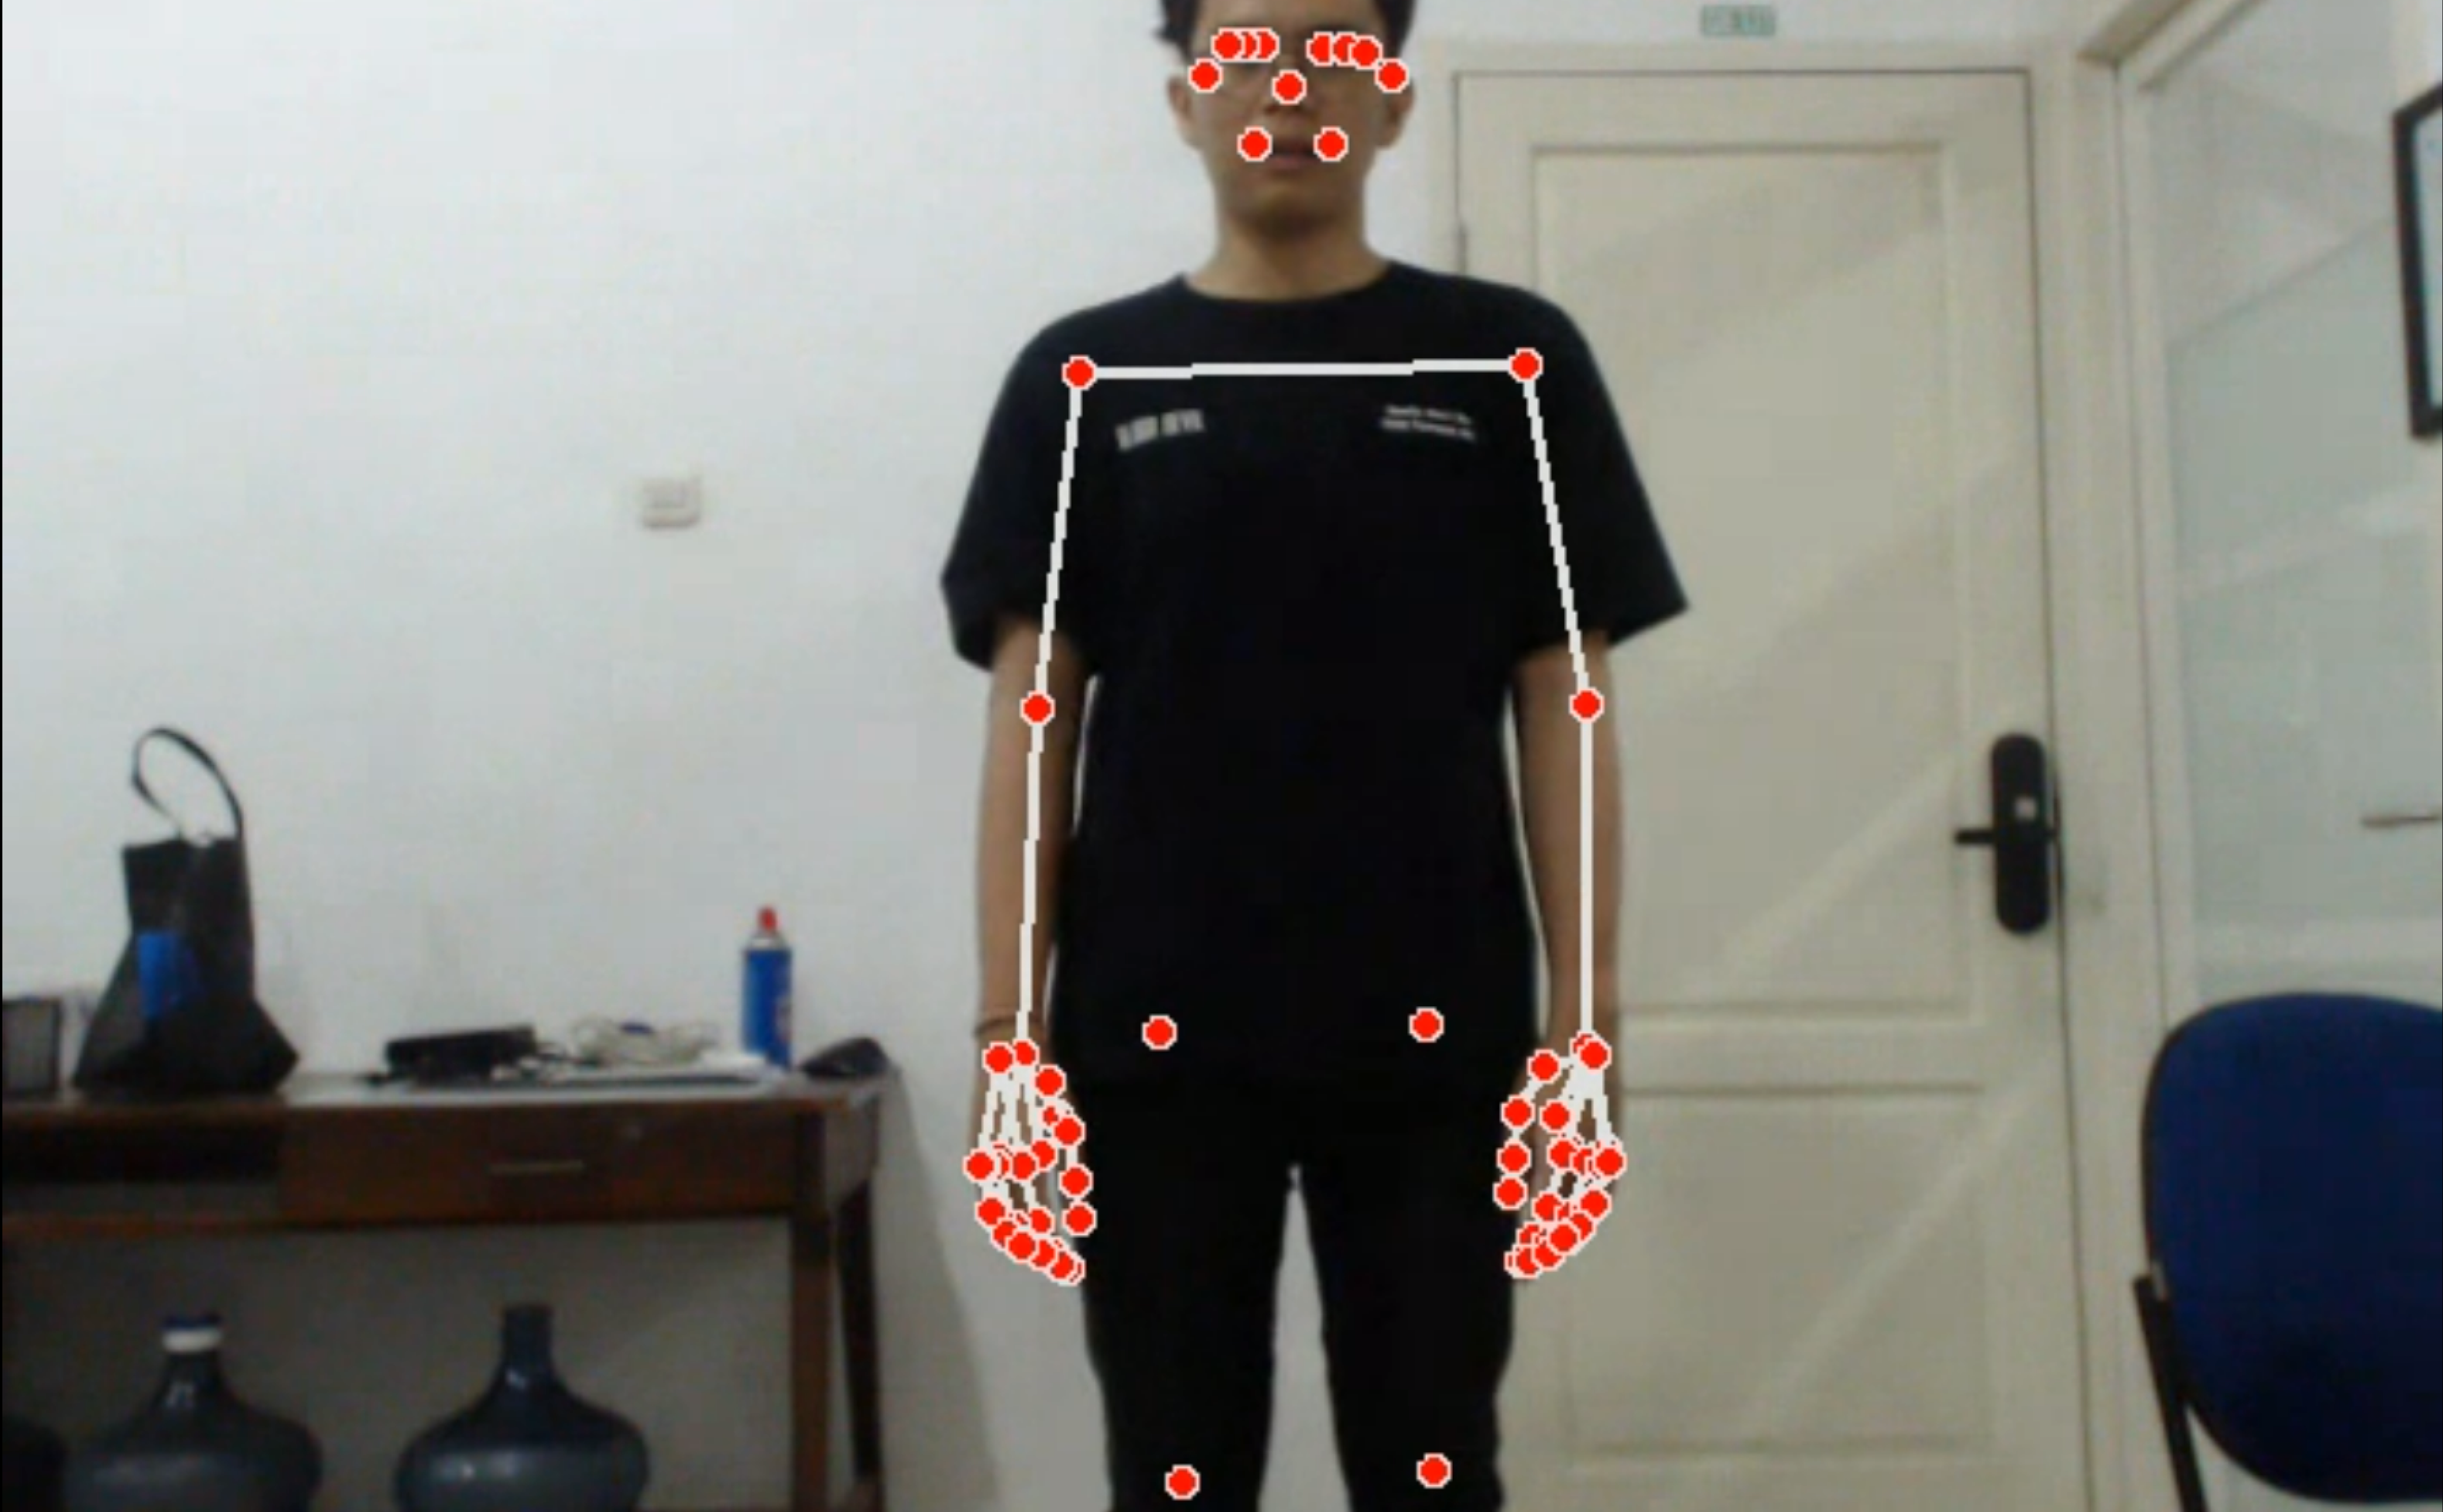
\includegraphics[scale=0.15]{gambar/bab4-jarak300.png}                \\
  \hline
  240 cm            & 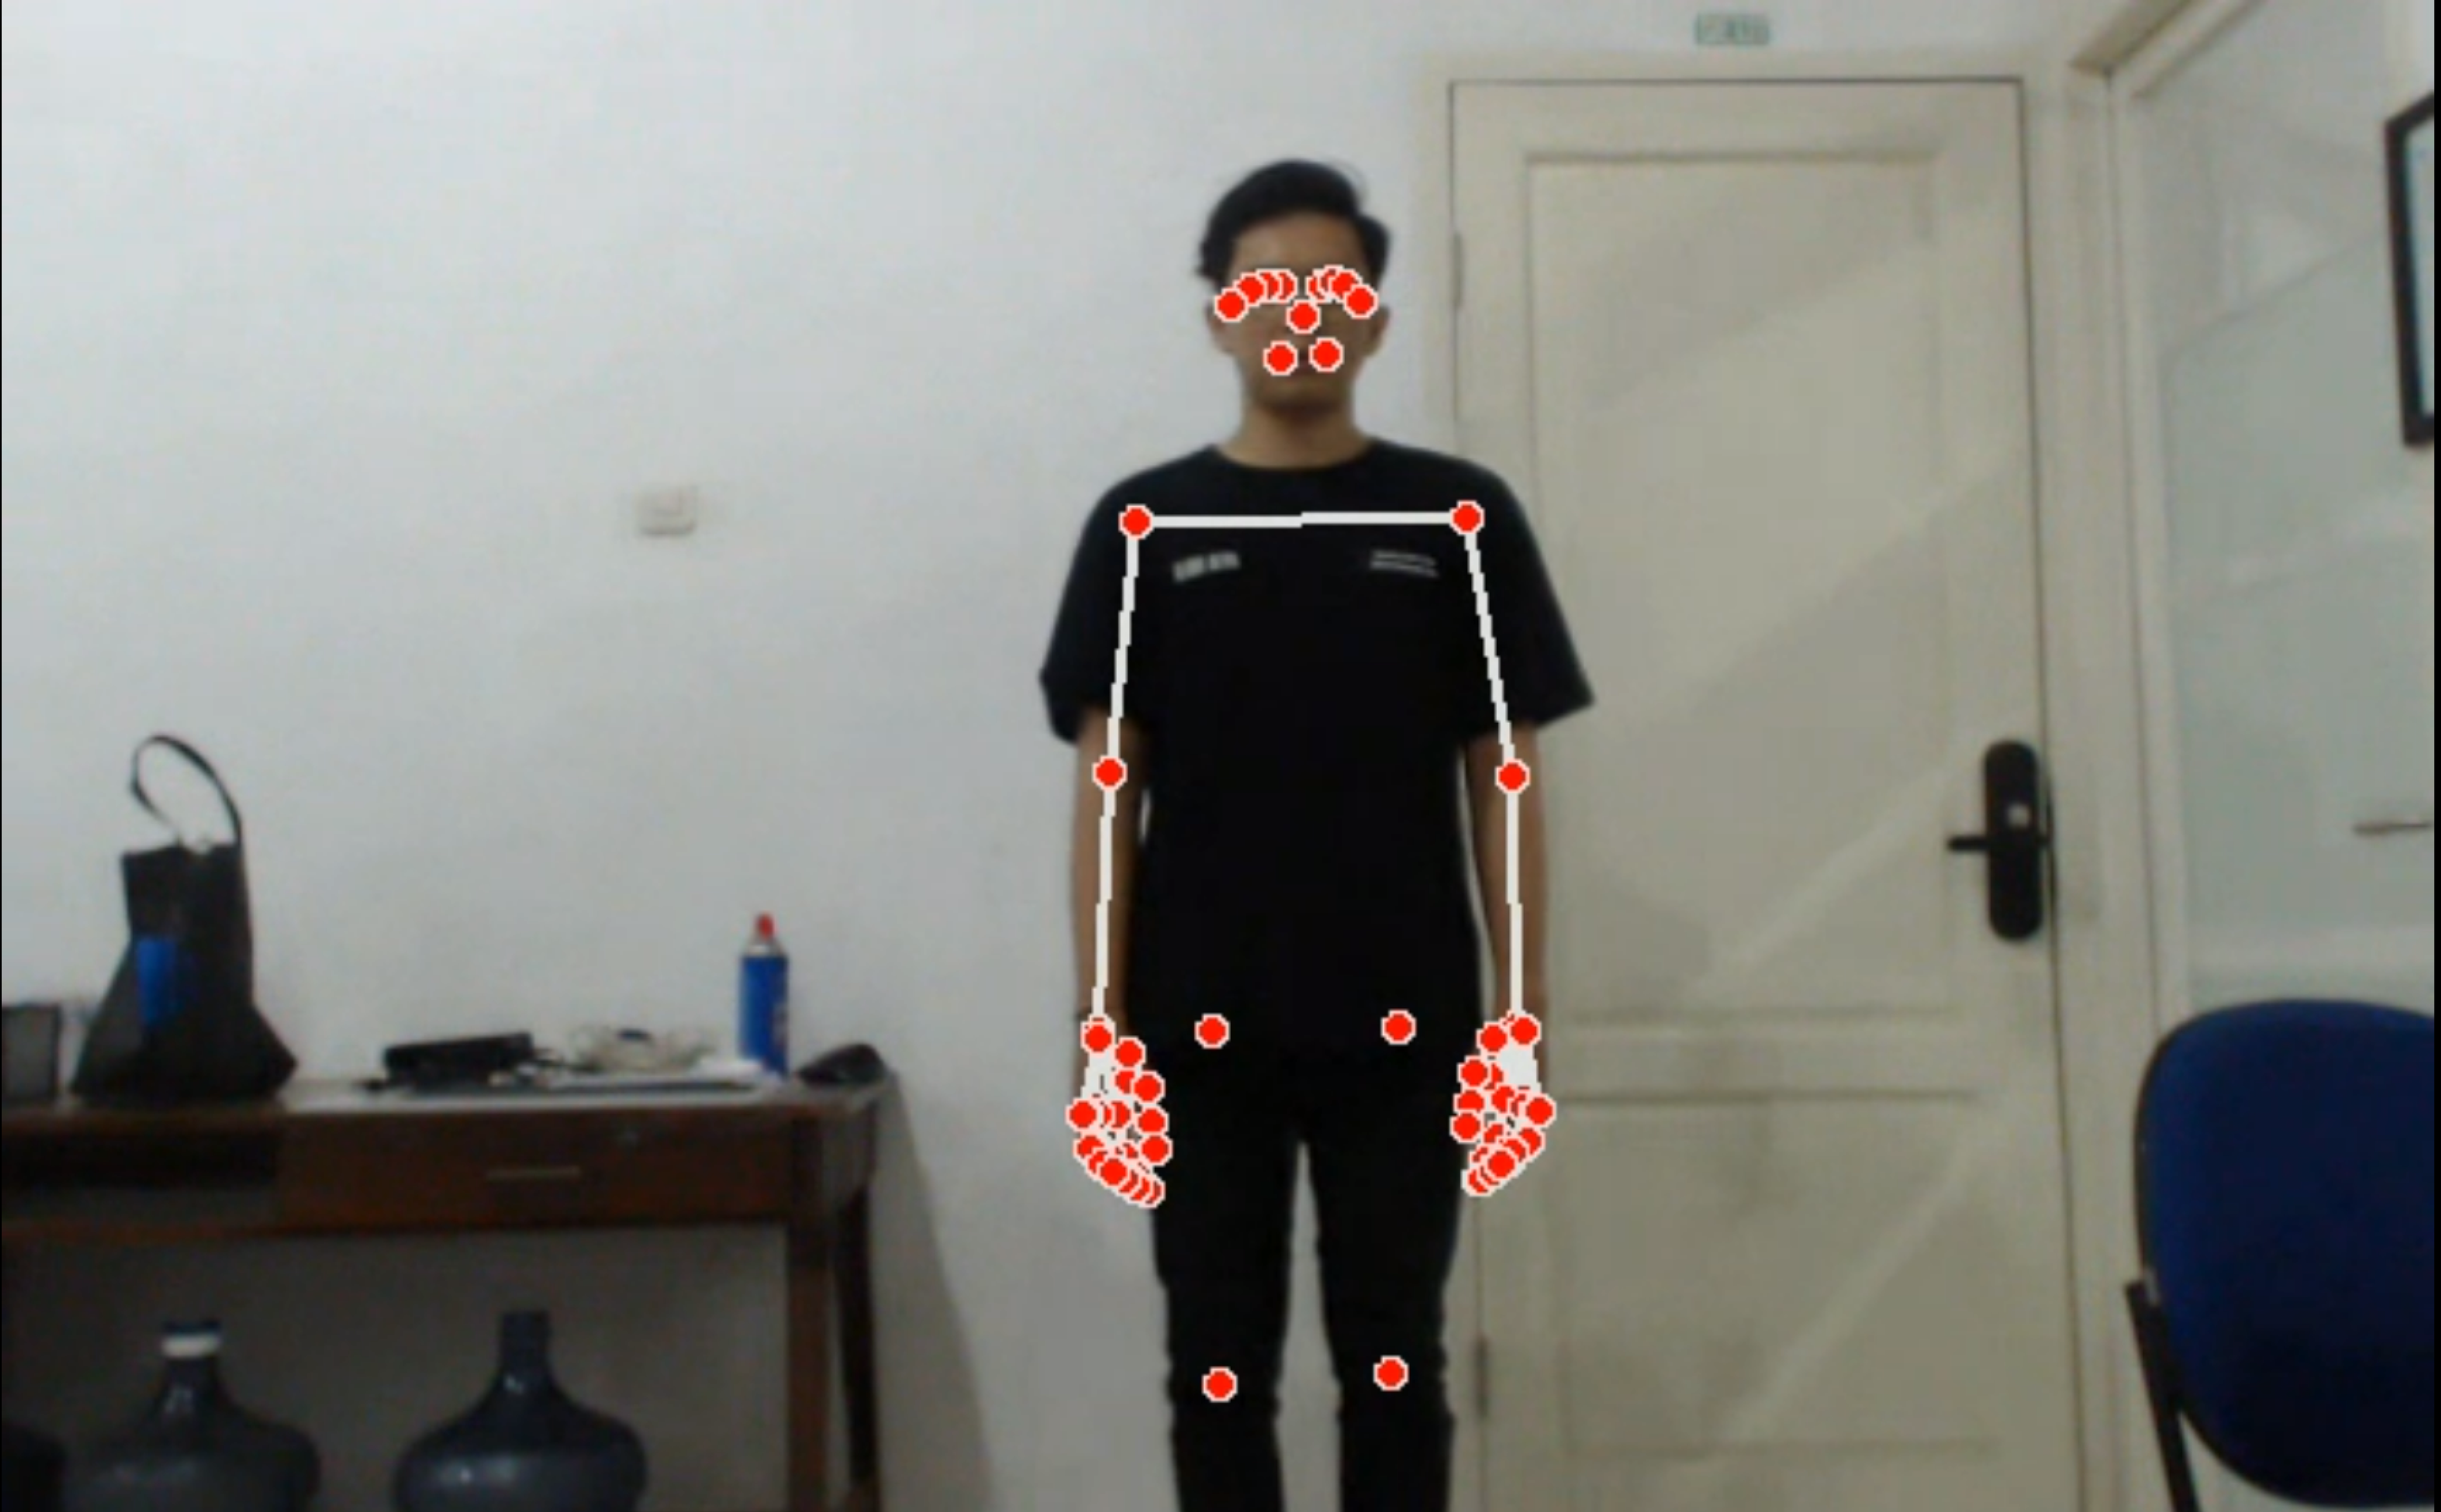
\includegraphics[scale=0.15]{gambar/bab4-jarak240.png}                 \\
  \hline
  300 cm            & 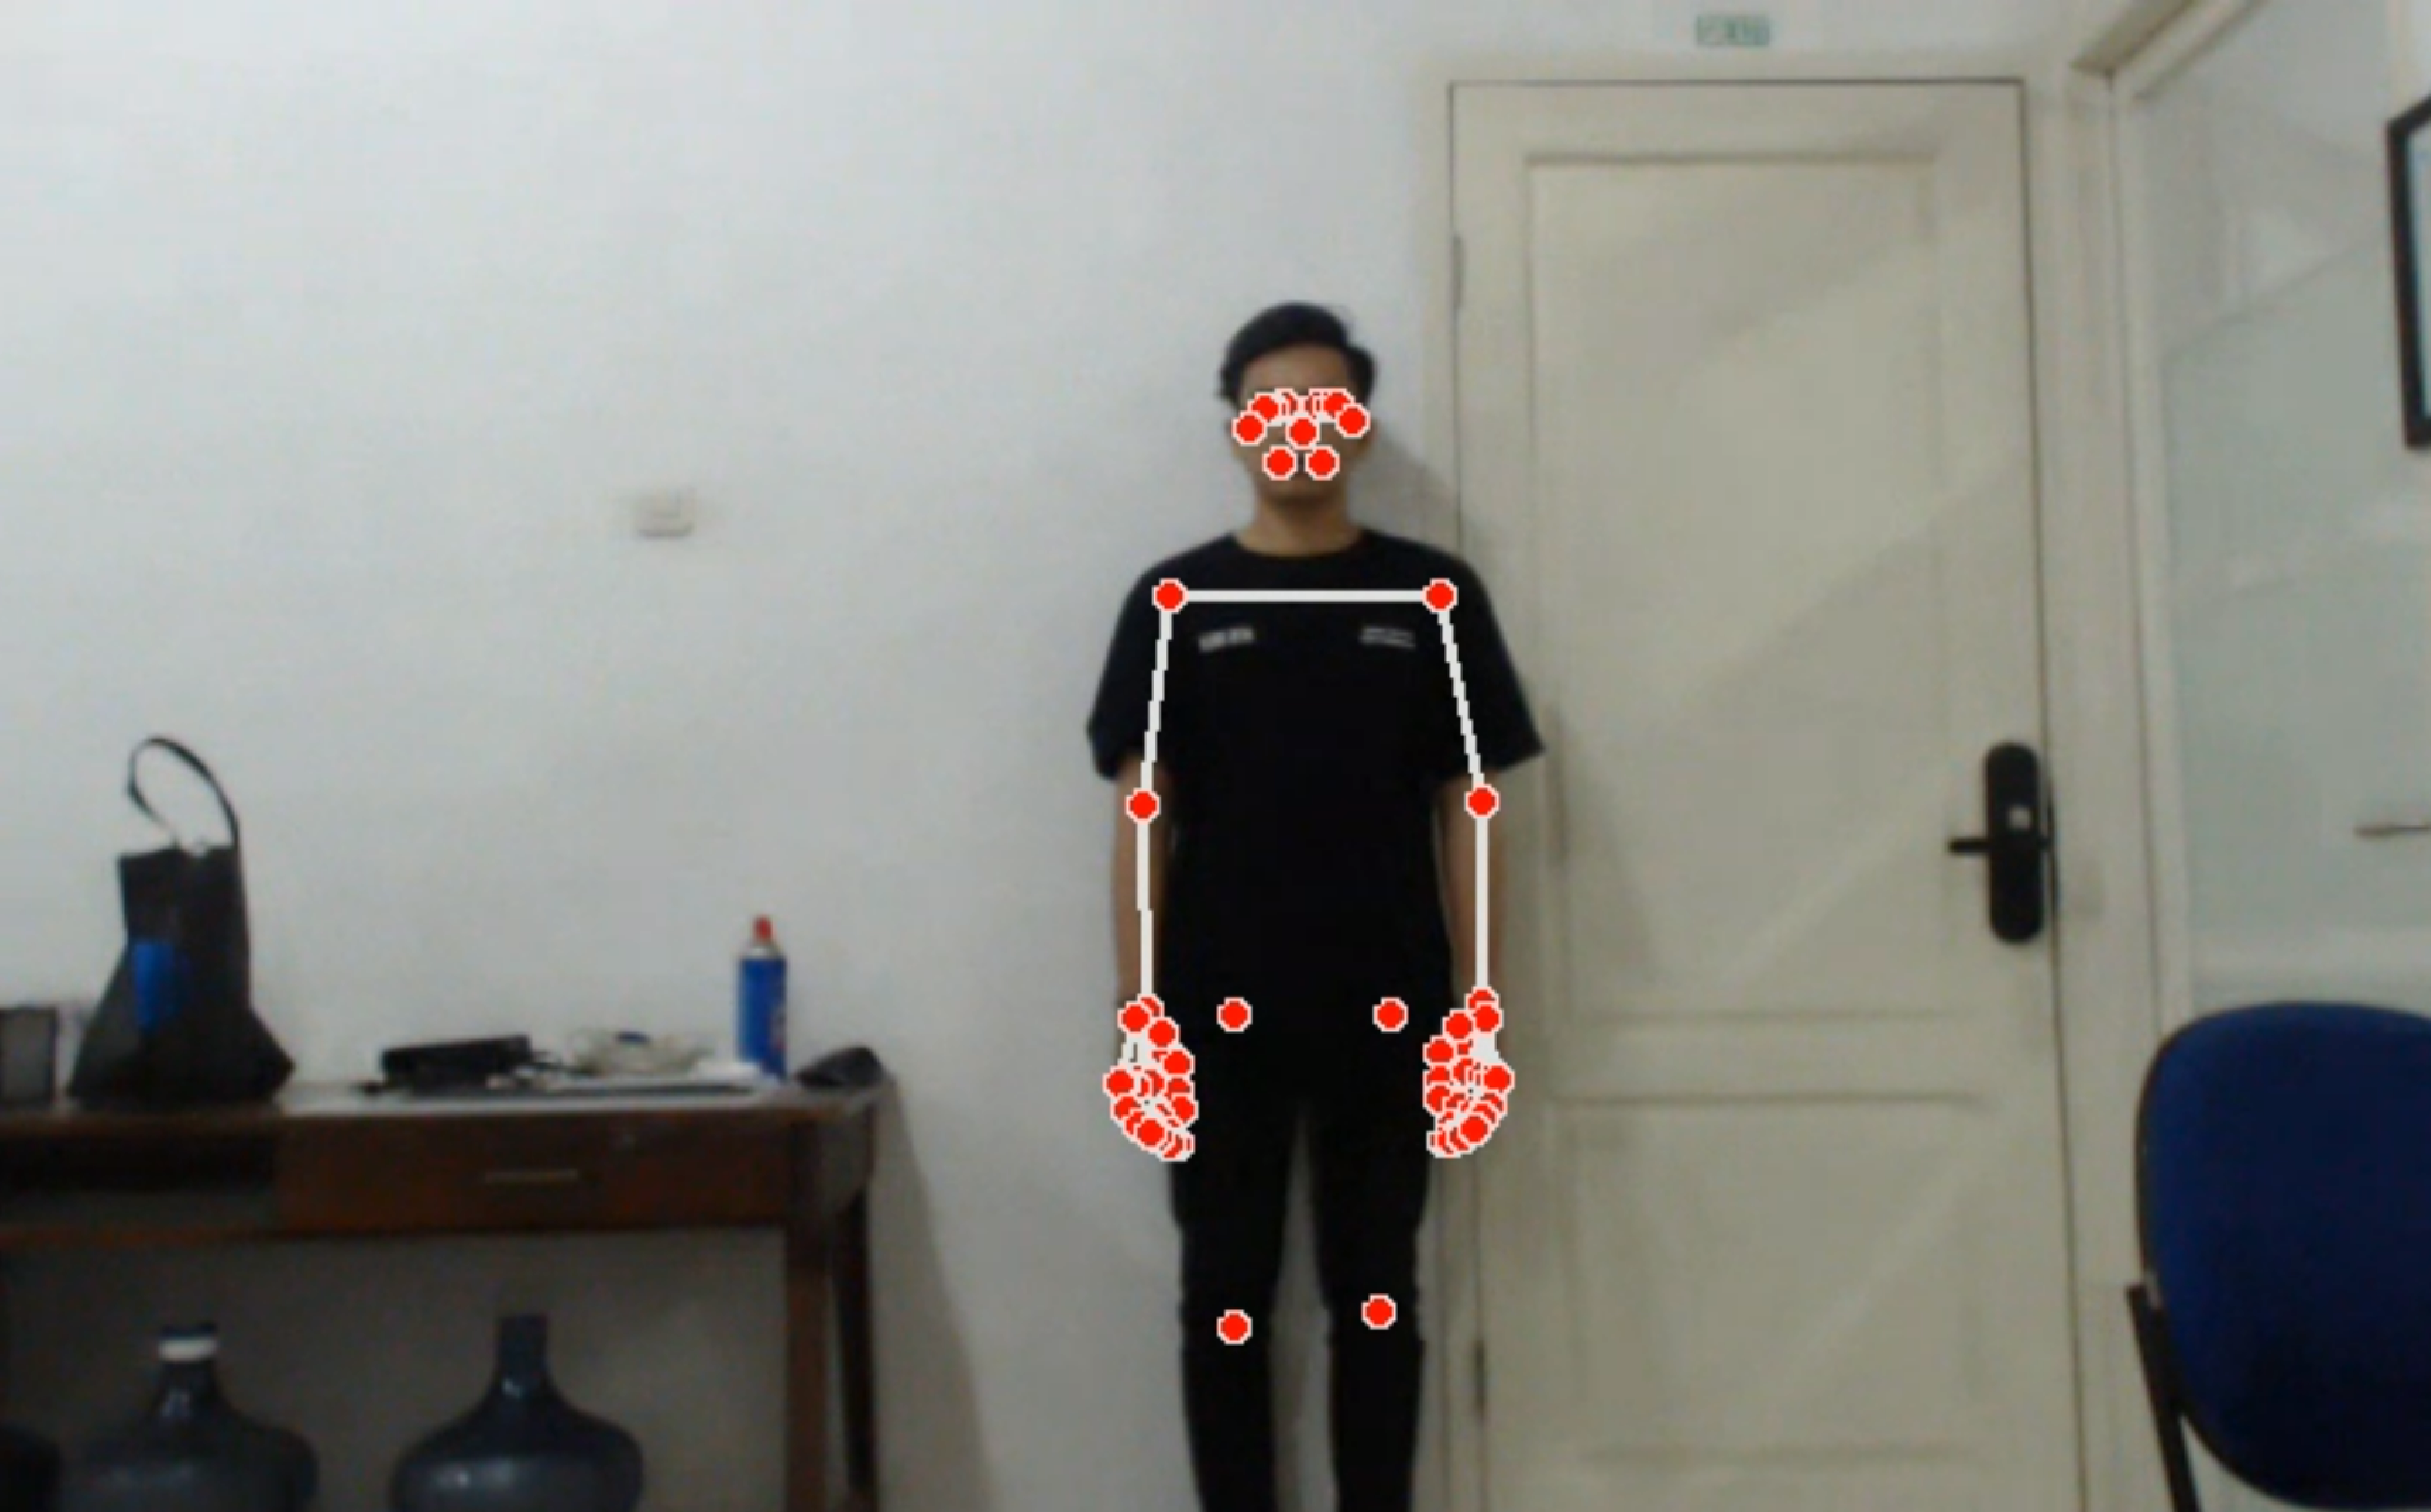
\includegraphics[scale=0.15]{gambar/bab4-jarak180.png}                 \\
  \hline
\end{longtable}

Pada pengujian kondisi jarak ini dilakukan untuk memahami bagaimana performa model pada jarak kamera dengan pengguna yang berbeda - beda. Adapun jarak yang akan digunakan pada pengujian ini adalah 180 cm, 240 cm, dan 300 cm. Variasi jarak ini dipilih dengan mempertimbangkan bahwa bagian kepala hingga tangan pengguna dapat terlihat secara jelas pada kamera sehingga setiap gerakan bahasa isyarat yang akan dilakukan. Untuk menghasilkan klasifikasi model diperlukan 30 \emph{frame} dan untuk setiap \emph{frame} diekstraksi koordinatnya dengan menggunakan \emph{framework} Mediapipe, apabila bagian tubuh pengguna (terkhususnya tangan dan kepala yang dominan digunakan untuk merepresentasikan suatu bahasa isyarat) tidak terlihat pada kamera akan mempengaruhi data koordinat yang didapatkan dan menyulitkan model untuk melakukan klasifikasi dengan tepat. Adapun posisi pengguna dengan jarak masing - masing dapat dlihat pada tabel \ref{tb:kondisijarak}. 

Model penerjemah bahasa Indonesia (BISINDO) yang akan digunakan pada pengujian ini adalah model pada bagian \ref{sec:analisismodel3} karena merupakan model yang menghasilkan klasifikasi yang terbaik jika dibandingkan dengan model lainnya. Untuk setiap variasi jarak akan dilakukan pengujian sebanyak tiga kali dengan kondisi ruangan yang memiliki intensitas cahaya yang terang (berkisar pada 125 lux). Pada setiap pengujian akan dicari hasil klasifikasi model, waktu yang dibutuhkan model untuk menghasilkan klasifikasi bahasa isyarat berdasarkan data koordinat yang diberikan(\emph{processing time}), dan waktu total yang dibutuhkan dalam menghasilkan klasifikasi bahasa isyarat (\emph{complete time}).  

\subsection{Pengujian Jarak 180 cm}
\label{sec:analisisjarak1}

\begin{longtable}{|c|c|c|c|}
  \caption{Pengujian Pertama Model di Kondisi Jarak 180 cm}
  \label{tb:prediksipendek1}                                   \\
  \hline
  \rowcolor[HTML]{C0C0C0}
  \textbf{Kosakata} & \textbf{Klasifikasi Model} & \textbf{\emph{Processing Time}} & \textbf{\emph{Complete Time}}\\
  \hline
  Maaf              & Maaf                          & 0.09432005882263184 detik                          & 2.6262545585632324 detik                                 \\
  Tolong            & Tolong                        & 0.09578323364257812 detik                          & 2.7582406997680664 detik                                 \\
  Nama              & Nama                          & 0.0936741828918457 detik                           & 2.7642273902893066 detik                                 \\
  Saya              & Saya                          & 0.09214234352111816 detik                          & 1.4595723152160645 detik                                 \\
  Siapa              & Siapa                        & 0.09187936782836914 detik                          & 2.6860642433166504 detik                                 \\
  Rumah             & \textcolor{red}{Delete}       & 0.09518122673034668 detik                          & 2.7240443229675293 detik                                 \\
  Delete            & Delete                        & 0.09378981590270996 detik                          & 1.4715027809143066 detik                                 \\
  Standby           & Standby                       & 0.09064006805419922 detik                          & 1.4081025123596191 detik                                 \\
  Translate         & Translate                     & 0.09035801887512207 detik                          & 2.901949882507324 detik                                \\
  \hline
\end{longtable}

\begin{longtable}{|c|c|c|c|}
  \caption{Pengujian Kedua Model di Kondisi Jarak 180 cm}
  \label{tb:prediksipendek2}                                   \\
  \hline
  \rowcolor[HTML]{C0C0C0}
  \textbf{Kosakata} & \textbf{Klasifikasi Model} & \textbf{\emph{Processing Time}} & \textbf{\emph{Complete Time}}\\
  \hline
  Maaf              & \textcolor{red}{Tolong}       & 0.1025094985961914  detik                           & 2.683281898498535  detik                                 \\
  Tolong            & Tolong                        & 0.10531425476074219 detik                           & 2.6761865615844727 detik                                  \\
  Nama              & Nama                          & 0.10347270965576172 detik                           & 2.837998867034912  detik                                 \\
  Saya              & Saya                          & 0.10077977180480957 detik                           & 1.6065859794616701 detik                                  \\
  Siapa              & Siapa                        & 0.09792852401733398 detik                           & 2.89107084274292   detik                                \\
  Rumah             & Rumah                         & 0.09961485862731934 detik                           & 2.9763364791870117 detik                                  \\
  Delete            & Delete                        & 0.10204243659973145 detik                           & 1.4318633079528809 detik                                  \\
  Standby           & Standby                       & 0.10916757583618164 detik                           & 1.4253973960876465 detik                                  \\
  Translate         & Translate                     & 0.1098337173461914  detik                           & 3.0064201354980464 detik                                  \\
  \hline
\end{longtable}

\newpage
\begin{longtable}{|c|c|c|c|}
  \caption{Pengujian Ketiga Model di Kondisi Jarak 180 cm}
  \label{tb:prediksipendek3}                                   \\
  \hline
  \rowcolor[HTML]{C0C0C0}
  \textbf{Kosakata} & \textbf{Klasifikasi Model} & \textbf{\emph{Processing Time}} & \textbf{\emph{Complete Time}}\\
  \hline
  Maaf              & Maaf                          & 0.09703993797302246 detik                          & 2.6079654693603516 detik                                  \\
  Tolong            & Tolong                        & 0.11110496520996094 detik                          & 2.688016891479492 detik                                \\
  Nama              & Nama                          & 0.11299991607666016 detik                          & 2.854478359222412 detik                                \\
  Saya              & Saya                          & 0.1057591438293457 detik                           & 1.4061927795410156 detik                                 \\
  Siapa             & Siapa                         & 0.10792779922485352 detik                          & 2.819080352783203 detik                                \\
  Rumah             & Rumah                         & 0.10235428810119629 detik                          & 2.8994321823120117 detik                                 \\
  Delete            & Delete                        & 0.10874819755554199 detik                          & 1.3875889778137207 detik                                 \\
  Standby           & Standby                       & 0.11034560203552246 detik                          & 1.3965654373168945 detik                                 \\
  Translate         & Translate                     & 0.10168957710266113 detik                          & 3.110654354095459 detik                                \\
  \hline
\end{longtable}

Berdasarkan tiga pengujian yang dilakukan, didapatkan bahwa hampir keseluruhan klasifikasi model yang sesuai dengan \emph{class} kosakata. Namun, terdapat beberapa kesalahan model dalam melakukan klasifikasi. Dapat dilihat pada tabel \ref{tb:prediksipendek1} untuk isyarat kosakata "Rumah" diklasifikasikan sebagai "Delete" dan pada tabel \ref{tb:prediksipendek2} untuk isyarat kosakata "Maaf" diklasifikasikan sebagai "Tolong". Adanya kemiripan antara kosakata menjadi penyebab utama terjadinya kesalahan ini. Kosakata "Rumah" dan "Delete" memiliki kemiripan pada gerakan isyaratnya, dimana kedua kosakata ini sama - sama menggunakan dua tangan dengan gerakan yang mayoritas terjadi pada bagian badan pengguna. Sedangkan untuk kosakata "Maaf" dan "Tolong" memiliki kemiripan pada gerakan isyaratnya dengan kedua kosakata sama - sama menggunakan tangan kanan dengan gerakan akhir yang mayoritas terjadi pada bagian samping wajah pengguna. Namun kemiripan ini tidak sepenuhnya membuat hasil klasifikasi menjadi lebih condong ke suatu kosakata, melainkan dengan pengguna yang memperagakan bahasa isyarat dengan mengutamakan "ciri khas" dari masing - masing bahasa isyarat dapat menghasilkan hasil klasifikasi model yang baik. Hal ini dapat dilihat pada tabel \ref{tb:prediksipendek2} menghasilkan keseluruhan klasifikasi yang benar untuk seluruh \emph{class} kosakata. Pada pengujian dengan kondisi jarak 180 cm, berdasarkan data pda tabel \ref{tb:prediksipendek1}, tabel tabel \ref{tb:prediksipendek2}, dan tabel tabel \ref{tb:prediksipendek3} menunjukkan bahwa model memiliki akurasi klasifikasi sebesar 92.5\%.

Apabila dilihat berdasarkan waktu pemrosesan, rata - rata waktu yang dibutuhkan model untuk menghasilkan klasifikasi bahasa isyarat (\emph{processing time}) adalah 0.101 detik dan rata - rata waktu yang dibutuhkan dalam menghasilkan klasifikasi bahasa isyarat (\emph{complete time}) adalah 2.352 detik. Berdasakan data ini, dapat diamati bahwa model memerlukan waktu yang terbilang singkat dalam memproses serangkaian data koordinat yang diberikan dengan program penerjemah yang mampu menyelesaikan proses klasifikasi dengan cepat untuk sistem yang berjalan secara \emph{real time}. Meskipun dengan kondisi pengguna yang memiliki jarak yang cukup dekat dengan kamera, tidak mempengaruhi secara signifikan terhadap proses klasifikasi bahasa isyarat yang dilakukan oleh model.

Pada pengujian di kondisi jarak 180 cm ini, perlu diperhatikan bahwa pengguna harus melakukan gerakan bahasa isyarat dengan memastikan bahwa bagian tubuh kepala hingga tangan dengan jelas terlihat. Hal ini sangat krusial karena model memerlukan informasi koordinat yang lengkap untuk setiapp gerakan isyarat sehingga dapat menghasilkan klasifikasi yang tepat. Terkhususnya untuk kosakata "Translate", "Maaf", "Tolong", dan "Delete" yang memiliki gerakan isyarat yang cukup dinamis dan mayoritas gerakannya terjadi di samping kepala pengguna.  

\newpage
\subsection{Pengujian Jarak 240 cm}
\label{sec:analisisjarak2}

\begin{longtable}{|c|c|c|c|}
  \caption{Pengujian Pertama Model di Kondisi Jarak 240 cm}
  \label{tb:prediksitengah1}                                   \\
  \hline
  \rowcolor[HTML]{C0C0C0}
  \textbf{Kosakata} & \textbf{Klasifikasi Model} & \textbf{\emph{Processing Time}} & \textbf{\emph{Complete Time}}\\
  \hline
  Maaf              & Maaf                        & 0.09363484382629395 detik                           & 2.8636908531188965 detik                                  \\
  Tolong            & Tolong                      & 0.09594297409057617 detik                           & 2.699732780456543 detik                                \\
  Nama              & Nama                        & 0.0991525650024414 detik                            & 2.716062068939209 detik                                \\
  Saya              & Saya                        & 0.09490489959716797 detik                           & 1.3848638534545898 detik                                 \\
  Siapa             & Siapa                       & 0.09771037101745605 detik                           & 2.778289318084717 detik                                \\
  Rumah             & Rumah                       & 0.09178900718688965 detik                           & 2.8422188758850098 detik                                 \\
  Delete            & Delete                      & 0.09782981872558594 detik                           & 2.746889591217041 detik                                \\
  Standby           & Standby                     & 0.09716463088989258 detik                           & 1.4444875717163086 detik                                 \\
  Translate         & Translate                   & 0.0946202278137207 detik                            & 2.8994321823120117 detik                                 \\
  \hline
\end{longtable}

\begin{longtable}{|c|c|c|c|}
  \caption{Pengujian Kedua Model di Kondisi Jarak 240 cm}
  \label{tb:prediksitengah2}                                   \\
  \hline
  \rowcolor[HTML]{C0C0C0}
  \textbf{Kosakata} & \textbf{Klasifikasi Model} & \textbf{\emph{Processing Time}} & \textbf{\emph{Complete Time}}\\
  \hline
  Maaf              & Maaf                        & 0.10062599182128906 detik                          & 2.837040424346924 detik                                 \\
  Tolong            & Tolong                      & 0.10464692115783691 detik                          & 2.745509147644043 detik                                 \\
  Nama              & Nama                        & 0.0791633129119873 detik                           & 2.7147960662841797 detik                                  \\
  Saya              & Saya                        & 0.11030316352844238 detik                          & 1.4569830894470215 detik                                  \\
  Siapa             & Siapa                       & 0.09940838813781738 detik                          & 2.7176427841186523 detik                                  \\
  Rumah             & Rumah                       & 0.10739994049072266 detik                          & 2.7834320068359375 detik                                  \\
  Delete            & Delete                      & 0.10262727737426758 detik                          & 2.848219871520996 detik                                 \\
  Standby           & Standby                     & 0.10418152809143066 detik                          & 1.4255762100219727 detik                                  \\
  Translate         & Translate                   & 0.10814952850341797 detik                          & 2.913722991943359  detik                                 \\
  \hline
\end{longtable}

\begin{longtable}{|c|c|c|c|}
  \caption{Pengujian Ketiga Model di Kondisi Jarak 240 cm}
  \label{tb:prediksitengah3}                                   \\
  \hline
  \rowcolor[HTML]{C0C0C0}
  \textbf{Kosakata} & \textbf{Klasifikasi Model} & \textbf{\emph{Processing Time}} & \textbf{\emph{Complete Time}}\\
  \hline
  Maaf              & Maaf                          & 0.08161234855651855 detik                           & 2.9344153404235835 detik                                  \\
  Tolong            & Tolong                        & 0.10856509208679199 detik                           & 2.842411994934082 detik                                 \\
  Nama              & Nama                          & 0.08474326133728027 detik                           & 2.8757071495056152 detik                                  \\
  Saya              & Saya                          & 0.10568404197692871 detik                           & 1.7722105979919436 detik                                  \\
  Siapa              & Siapa                        & 0.10201120376586914 detik                           & 2.6211905479431152 detik                                  \\
  Rumah             & \textcolor{red}{Delete}       & 0.10468339920043945 detik                           & 2.7255606651306152 detik                                  \\
  Delete            & Delete                        & 0.1030888557434082 detik                            & 2.8281641006469727 detik                                  \\
  Standby           & Standby                       & 0.10799098014831543 detik                           & 1.4275431632995605 detik                                  \\
  Translate         & Translate                     & 0.10626840591430664 detik                           & 2.813551425933838 detik                                 \\
  \hline
\end{longtable}

Berdasarkan tiga pengujian yang telah dilakukan, didapatkan bahwa hampir keseluruhan klasifikasi model telah sesuai dengan \emph{class} kosakata yang bersesuaian. Hal ini menunjukkan bahwa adanya pengaruh antara jarak pengguna dengan kamera terhadap proses klasifikasi model. Peningkatan jarak pengguna terhadap menghasilkan klasifikasi yang lebih baik. Namun, masih terdapat kesalahan yang dapat dilihat pada tabel \ref{tb:prediksitengah3}, yaitu isyarat kosakata "Rumah" diklasifikasikan sebagai "Delete". Sama seperti yang sudah dijelaskan pada pengujian di kondisi jarak 180 cm bahwa terdapat kemiripan antara kosakata "Rumah" dengan "Delete". Pada pengujian dengan kondisi jarak 240 cm ini, berdasarkan data pada tabel \ref{tb:prediksitengah1}, tabel \ref{tb:prediksitengah2}, dan tabel \ref{tb:prediksitengah3} menunjukkan bahwa model memiliki akurasi klasifikasi sebesar 96.3\%.

Apabila dilihat berdasarkan waktu pemrosesan, rata - rata waktu yang dibutuhkan model untuk menghasilkan klasifikasi bahasa isyarat (\emph{processing time}) adalah 0.099 detik dan rata - rata waktu yang dibutuhkan dalam menghasilkan klasifikasi bahasa isyarat (\emph{complete time}) adalah 2.506 detik. Apabila dibandingkan dengan pengujian sebelumnya (kondisi jarak 180 cm). Terdapat peningkatan pada nilai \emph{processing time} seiring dengan peningkatan jarak kamera dengan pengguna yaitu sebesar 0.002 detik. Sedangkan untuk nilai \emph{complete time} mengalami penurunan seiring dengan peningkatan jarak kamera dengan pengguna, yaitu sebesar 0.154 detik. Hal ini dapat disebabkan oleh adanya pengaruh antara jarak pengguna dengan kamera terhadap bagaimana beban kerja kamera dalam menangkap tiap \emph{frame}.

\subsection{Pengujian Jarak 300 cm}
\label{sec:analisisjarak3}

\begin{longtable}{|c|c|c|c|}
  \caption{Pengujian Pertama Model di Kondisi Jarak 300 cm}
  \label{tb:prediksijauh1}                                   \\
  \hline
  \rowcolor[HTML]{C0C0C0}
  \textbf{Kosakata} & \textbf{Klasifikasi Model} & \textbf{\emph{Processing Time}} & \textbf{\emph{Complete Time}}\\
  \hline
  Maaf              & Maaf                          & 0.09520149230957031 detik                           & 2.738614082336426 detik                                  \\
  Tolong            & Tolong                        & 0.0926811695098877 detik                            & 2.878732681274414 detik                                  \\
  Nama              & Nama                          & 0.0982358455657959 detik                            & 2.915797233581543 detik                                  \\
  Saya              & Saya                          & 0.0943760871887207 detik                            & 2.8119421005249023 detik                                  \\
  Siapa              & Siapa                        & 0.1026923656463623 detik                            & 2.7649641036987305 detik                                  \\
  Rumah             & Rumah                         & 0.09520149230957031 detik                           & 2.740323543548584 detik                                  \\
  Delete            & Delete                        & 0.09269595146179199 detik                           & 2.981078624725342 detik                                  \\
  Standby           & Standby                       & 0.09149551391601562 detik                           & 2.813115119934082 detik                                  \\
  Translate         & Translate                     & 0.09415459632873535 detik                           & 2.848083972930908 detik                                  \\
  \hline
\end{longtable}

\begin{longtable}{|c|c|c|c|}
  \caption{Pengujian Kedua Model di Kondisi Jarak 300 cm}
  \label{tb:prediksijauh2}                                   \\
  \hline
  \rowcolor[HTML]{C0C0C0}
  \textbf{Kosakata} & \textbf{Klasifikasi Model} & \textbf{\emph{Processing Time}} & \textbf{\emph{Complete Time}}\\
  \hline
  Maaf              & Maaf                          & 0.11374950408935547 detik                           & 2.8633904457092285 detik                                  \\
  Tolong            & Tolong                        & 0.10336184501647949 detik                           & 2.7457737922668457 detik                                  \\
  Nama              & Nama                          & 0.1011803150177002 detik                            & 2.690098285675049 detik                                 \\
  Saya              & Saya                          & 0.11127400398254395 detik                           & 2.720317840576172 detik                                 \\
  Siapa              & Siapa                        & 0.10362887382507324 detik                           & 2.84954309463501 detik                                \\
  Rumah             & Rumah                         & 0.10374069213867188 detik                           & 2.8711438179016113 detik                                  \\
  Delete            & Delete                        & 0.10743093490600586 detik                           & 2.7329492568969727 detik                                  \\
  Standby           & Standby                       & 0.10061454772949219 detik                           & 2.903716564178467 detik                                 \\
  Translate         & Translate                     & 0.10336613655090332 detik                           & 2.752346992492676 detik                                 \\
  \hline
\end{longtable}

\newpage
\begin{longtable}{|c|c|c|c|}
  \caption{Pengujian Ketiga Model di Kondisi Jarak 300 cm}
  \label{tb:prediksijauh3}                                   \\
  \hline
  \rowcolor[HTML]{C0C0C0}
  \textbf{Kosakata} & \textbf{Klasifikasi Model} & \textbf{\emph{Processing Time}} & \textbf{\emph{Complete Time}}\\
  \hline
  Maaf              & Maaf                        & 0.09520149230957031 detik                          & 2.7579760551452637 detik                                 \\
  Tolong            & Tolong                      & 0.0926811695098877 detik                          & 2.6619672775268555 detik                                 \\
  Nama              & Nama                        & 0.0982358455657959 detik                          & 2.8861284255981445 detik                                 \\
  Saya              & Saya                        & 0.0943760871887207 detik                          & 2.800147533416748 detik                                 \\
  Siapa             & Siapa                       & 0.1026923656463623 detik                          & 2.763504981994629 detik                                 \\
  Rumah             & Rumah                       & 0.09520149230957031 detik                          & 2.811462879180908 detik                                  \\
  Delete            & Delete                      & 0.09269595146179199 detik                          & 2.6989388465881348 detik                                 \\
  Standby           & Standby                     & 0.09675002098083496 detik                          & 2.7558088302612305 detik                                  \\
  Translate         & Translate                   & 0.10323047637939453 detik                          & 2.67941951751709 detik                                  \\
  \hline
\end{longtable}

Berdasarkan tiga pengujian yang telah dilakukan, didapatkan bahwa keseluruhan klasifikasi model yang sesuai dengan \emph{class} kosakata. Hal ini menunjukkan bahwa peningkatan jarak berpengaruh pada proses klasifikasi yang dilakukan oleh model. Peningkatan jarak antara pengguna dengan kamera, terkhususnya pada jarak terjauh pada pengujian ini, menghasilkan klasifikasi yang lebih baik dan tepat sesuai dengan kosakata yang bersesuaian dengan gerakannya. Hal ini dapat disebabkan oleh semakin jauh jarak antara kamera dengan pengguna memudahkan dalam memproses pose pengguna sehingga menghasilkan data koordinat yang lebih baik lagi. Berdasarkan data pada tabel \ref{tb:prediksijauh1}, tabel \ref{tb:prediksijauh2}, tabel \ref{tb:prediksijauh3} menunjukkan bahwa model memiliki akurasi klasifikasi sebesar 100\%.

Apabila dilihat berdasarkan waktu pemrosesan, rata - rata waktu yang dibutuhkan model untuk menghasilkan klasifikasi bahasa isyarat (\emph{processing time}) adalah 0.099 detik dan rata - rata waktu yang dibutuhkan dalam menghasilkan klasifikasi bahasa isyarat (\emph{complete time}) adalah 2.794 detik. Dapat dilihat bahwa tidak terdapat peningkatan pada \emph{processing time} jika dibandingkan dengan variasi jarak pada pengujian sebelumnya. Namun, pada nilai \emph{complete time} terdapat penurunan jika dibandingkan dengan pengujian sebelumnya, yaitu sebesar 0.288 detik. Hal ini menunjukkan bahwa terdapat penurunan dari nilai \emph{complete time} seiring dengan peningkatan jarak kamera dengan pengguna. Hal ini dapat kembali lagi menguatkan bahwa adanya pengaruh antara jarak pengguna dengan kamera terhadap bagaimana beban kerja kamera dalam menangkap tiap \emph{frame}.

\subsection{Rangkuman Pengujian Kondisi Jarak}
\label{sec:analisisrangkumanjarak}

\begin{longtable}{|c|c|c|c|}
  \caption{Rangkuman Pengujian Kondisi Jarak}
  \label{tb:evaluasiJarak}                                   \\
  \hline
  \rowcolor[HTML]{C0C0C0}
  \textbf{Jarak} & \textbf{Akurasi} & \emph{\textbf{Avg. Processing Time}} & \emph{\textbf{Avg. Complete Time}} \\
  \hline
  180 cm & 0.89 & 0.1017 detik & 2.3660 detik \\
  240 cm & 0.96 & 0.0994 detik & 2.5098 detik \\
  300 cm & 1.00 & 0.0997 detik & 2.7918 detik \\
  \hline
\end{longtable}

Secara keseluruhan, dapat dilihat pada tabel \ref{tb:evaluasiJarak} bahwa variasi jarak yang berbeda tidak berpengaruh secara signifikan terhadap hasil klasifikasi model. Hal ini menunjukkan bahwa metode normalisasi data yang digunakan telah berhasil menghasilkan model yang invarian terhadap jarak. Dengan catatan bahwa posisi pengguna (terkhususnya bagian kepala dan tangan) dapat dengan jelas terlihat ketika melakukan gerakan isyarat. Dapat dilihat bahwa ada relasi antara jarak dengan \emph{average complete time}. Peningkatan \emph{average}. Namun, pada nilai \emph{average processing time} cenderung menurun dengan adanya peningkatan jarak. Kemampuan kamera dalam menangkap \emph{frame} menjadi pengaruh utama dalam peningkatan nilai \emph{complete time} dan \emph{processing time} karena gerakan isyarat yang dinamis memerlukan posisi kamera yang dapat menangkap setiap gerakan dengan jelas dan tepat. Semakin jelas gerakan isyarat yang ditangkap akan memudahkan \emph{framework} Mediapipe dalam mendapatkan data koordinat berdasarkan \emph{landmark} yang ada. Hal ini tentunya akan meningkatkan akurasi klasifikasi model, dimana ditunjukkan dengan adanya peningkatan akurasi seiring dengan peningkatan jarak.

\section{Pengujian Subjek Berbeda}
\label{sec:analisissubjek}

\begin{longtable}{|c|c|}
  \caption{Variasi Subjek Berbeda}
  \label{tb:kondisisubjek}                                   \\
  \hline
  \rowcolor[HTML]{C0C0C0}
  \textbf{Jenis Kelamin} & \textbf{Gambar Subjek}  \\
  \hline
  Perempuan            &  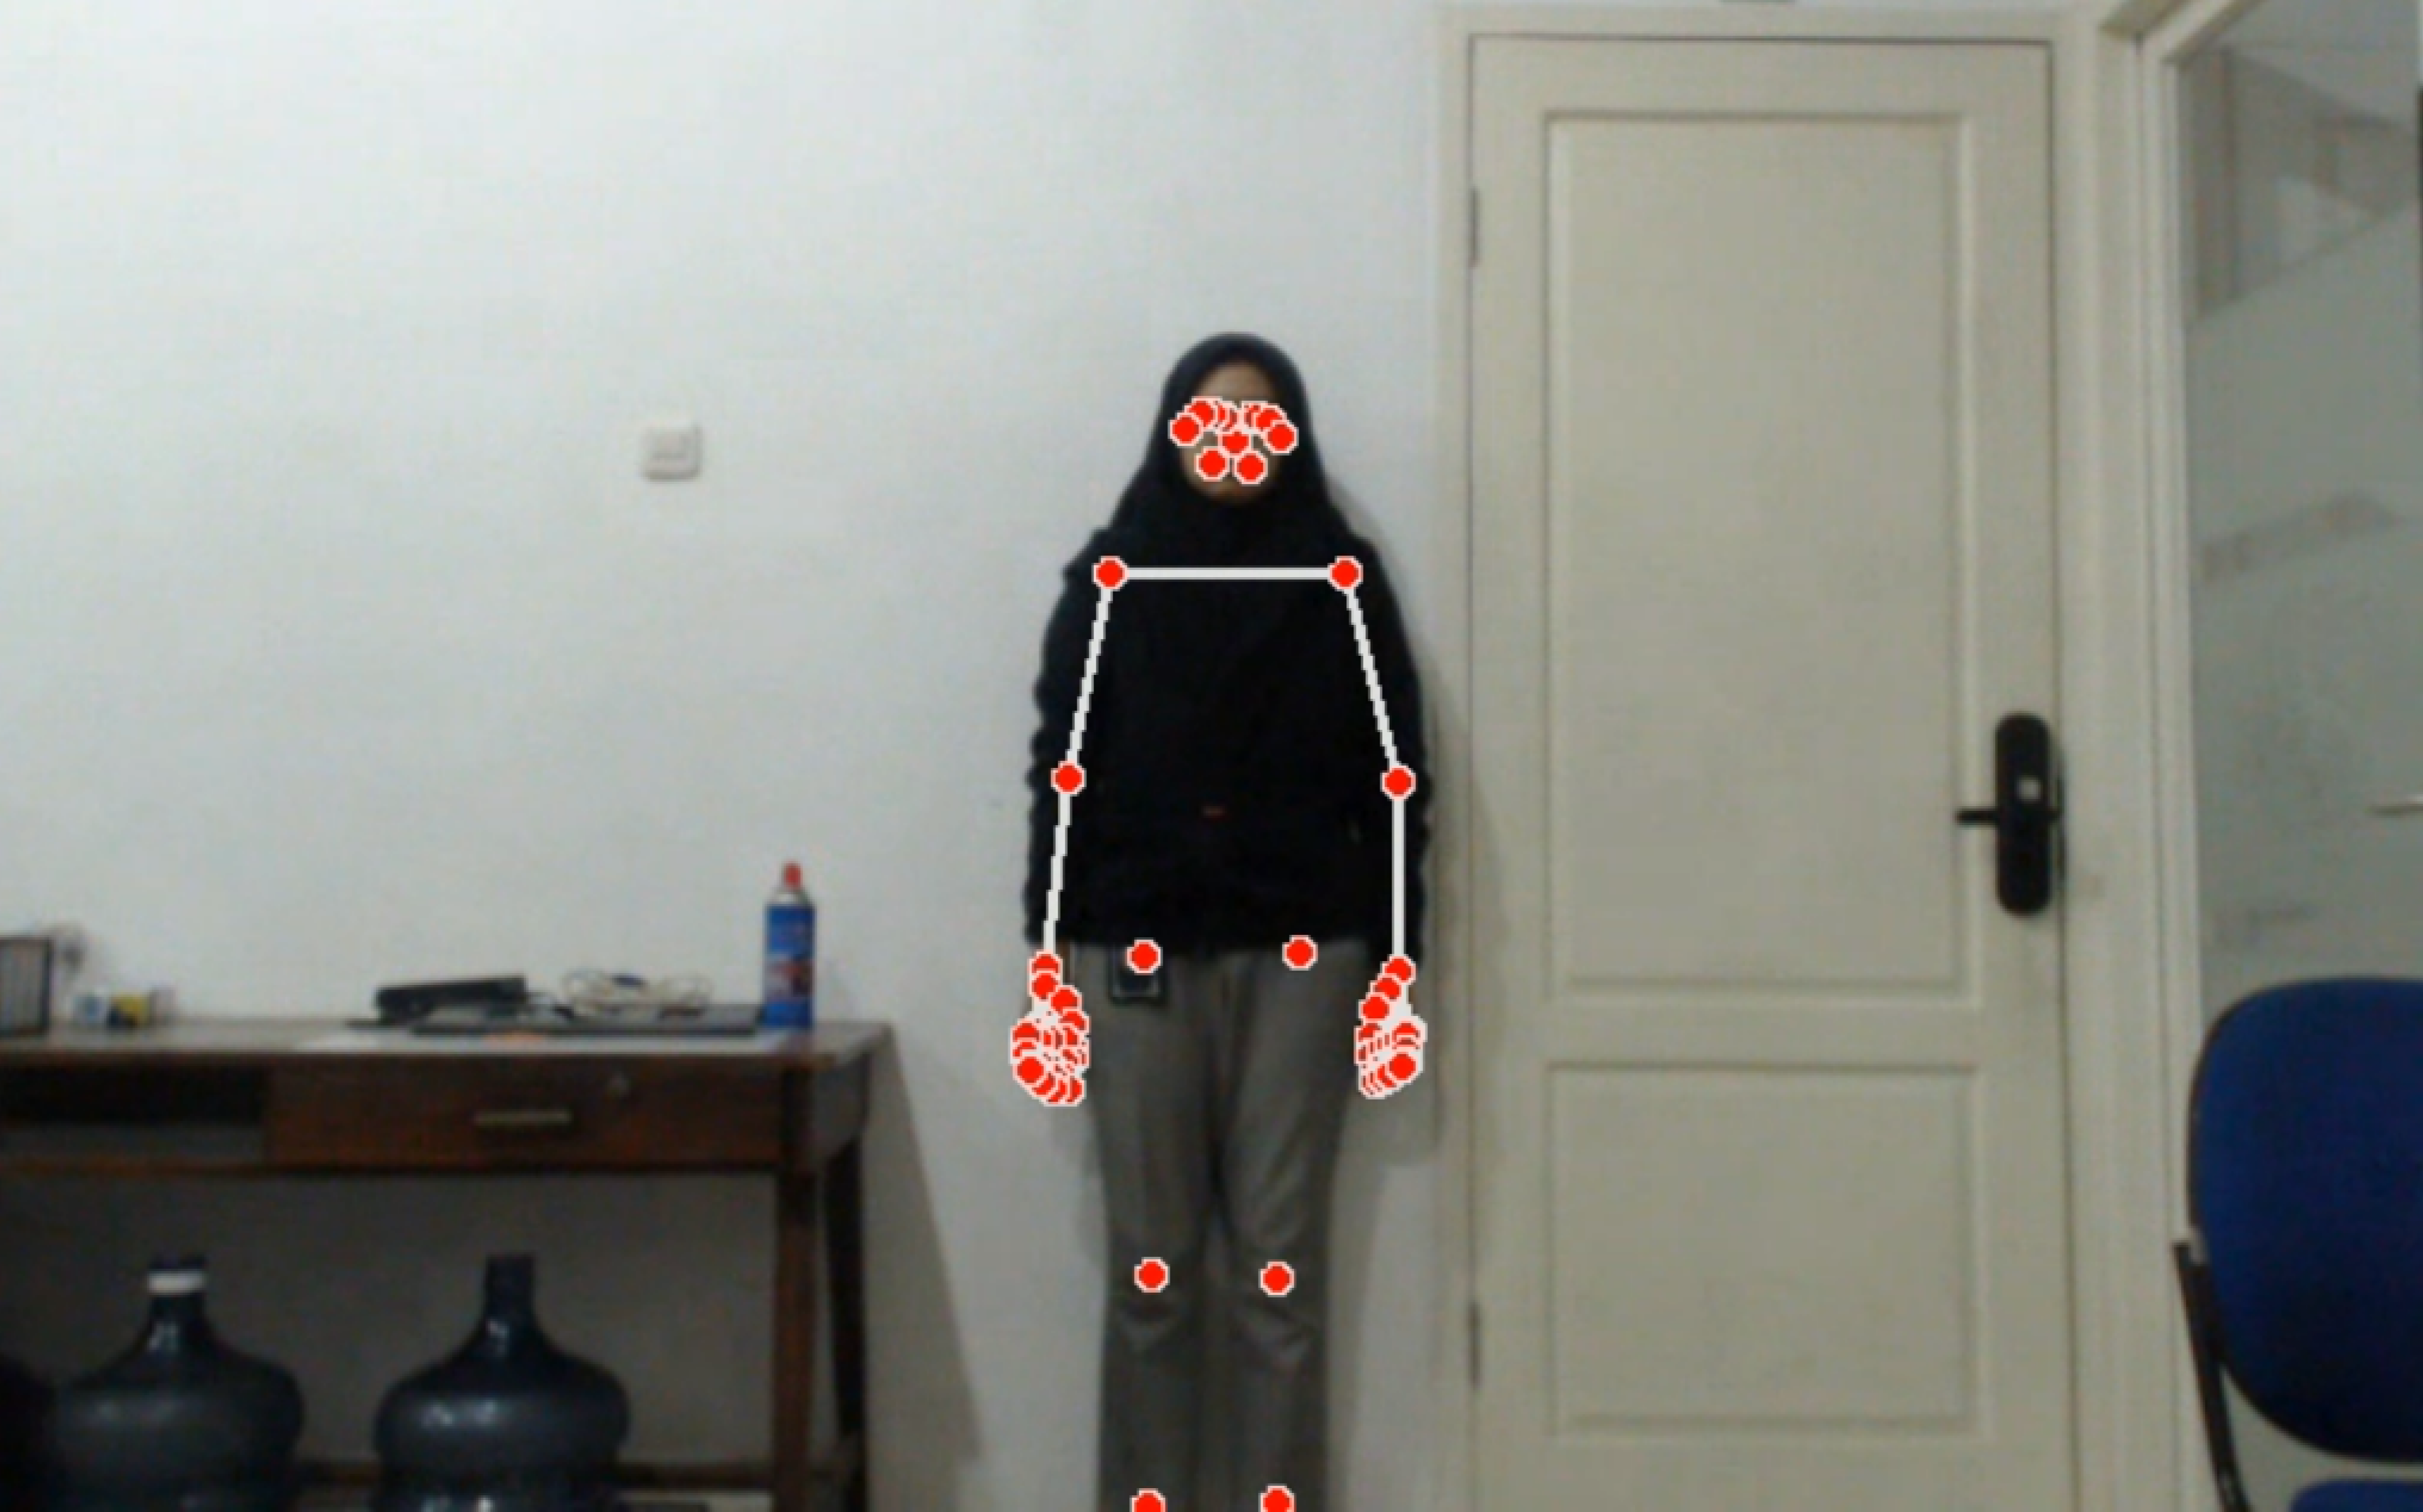
\includegraphics[scale=0.3]{gambar/bab4-rani.png}                \\
  \hline
  Laki - Laki            & 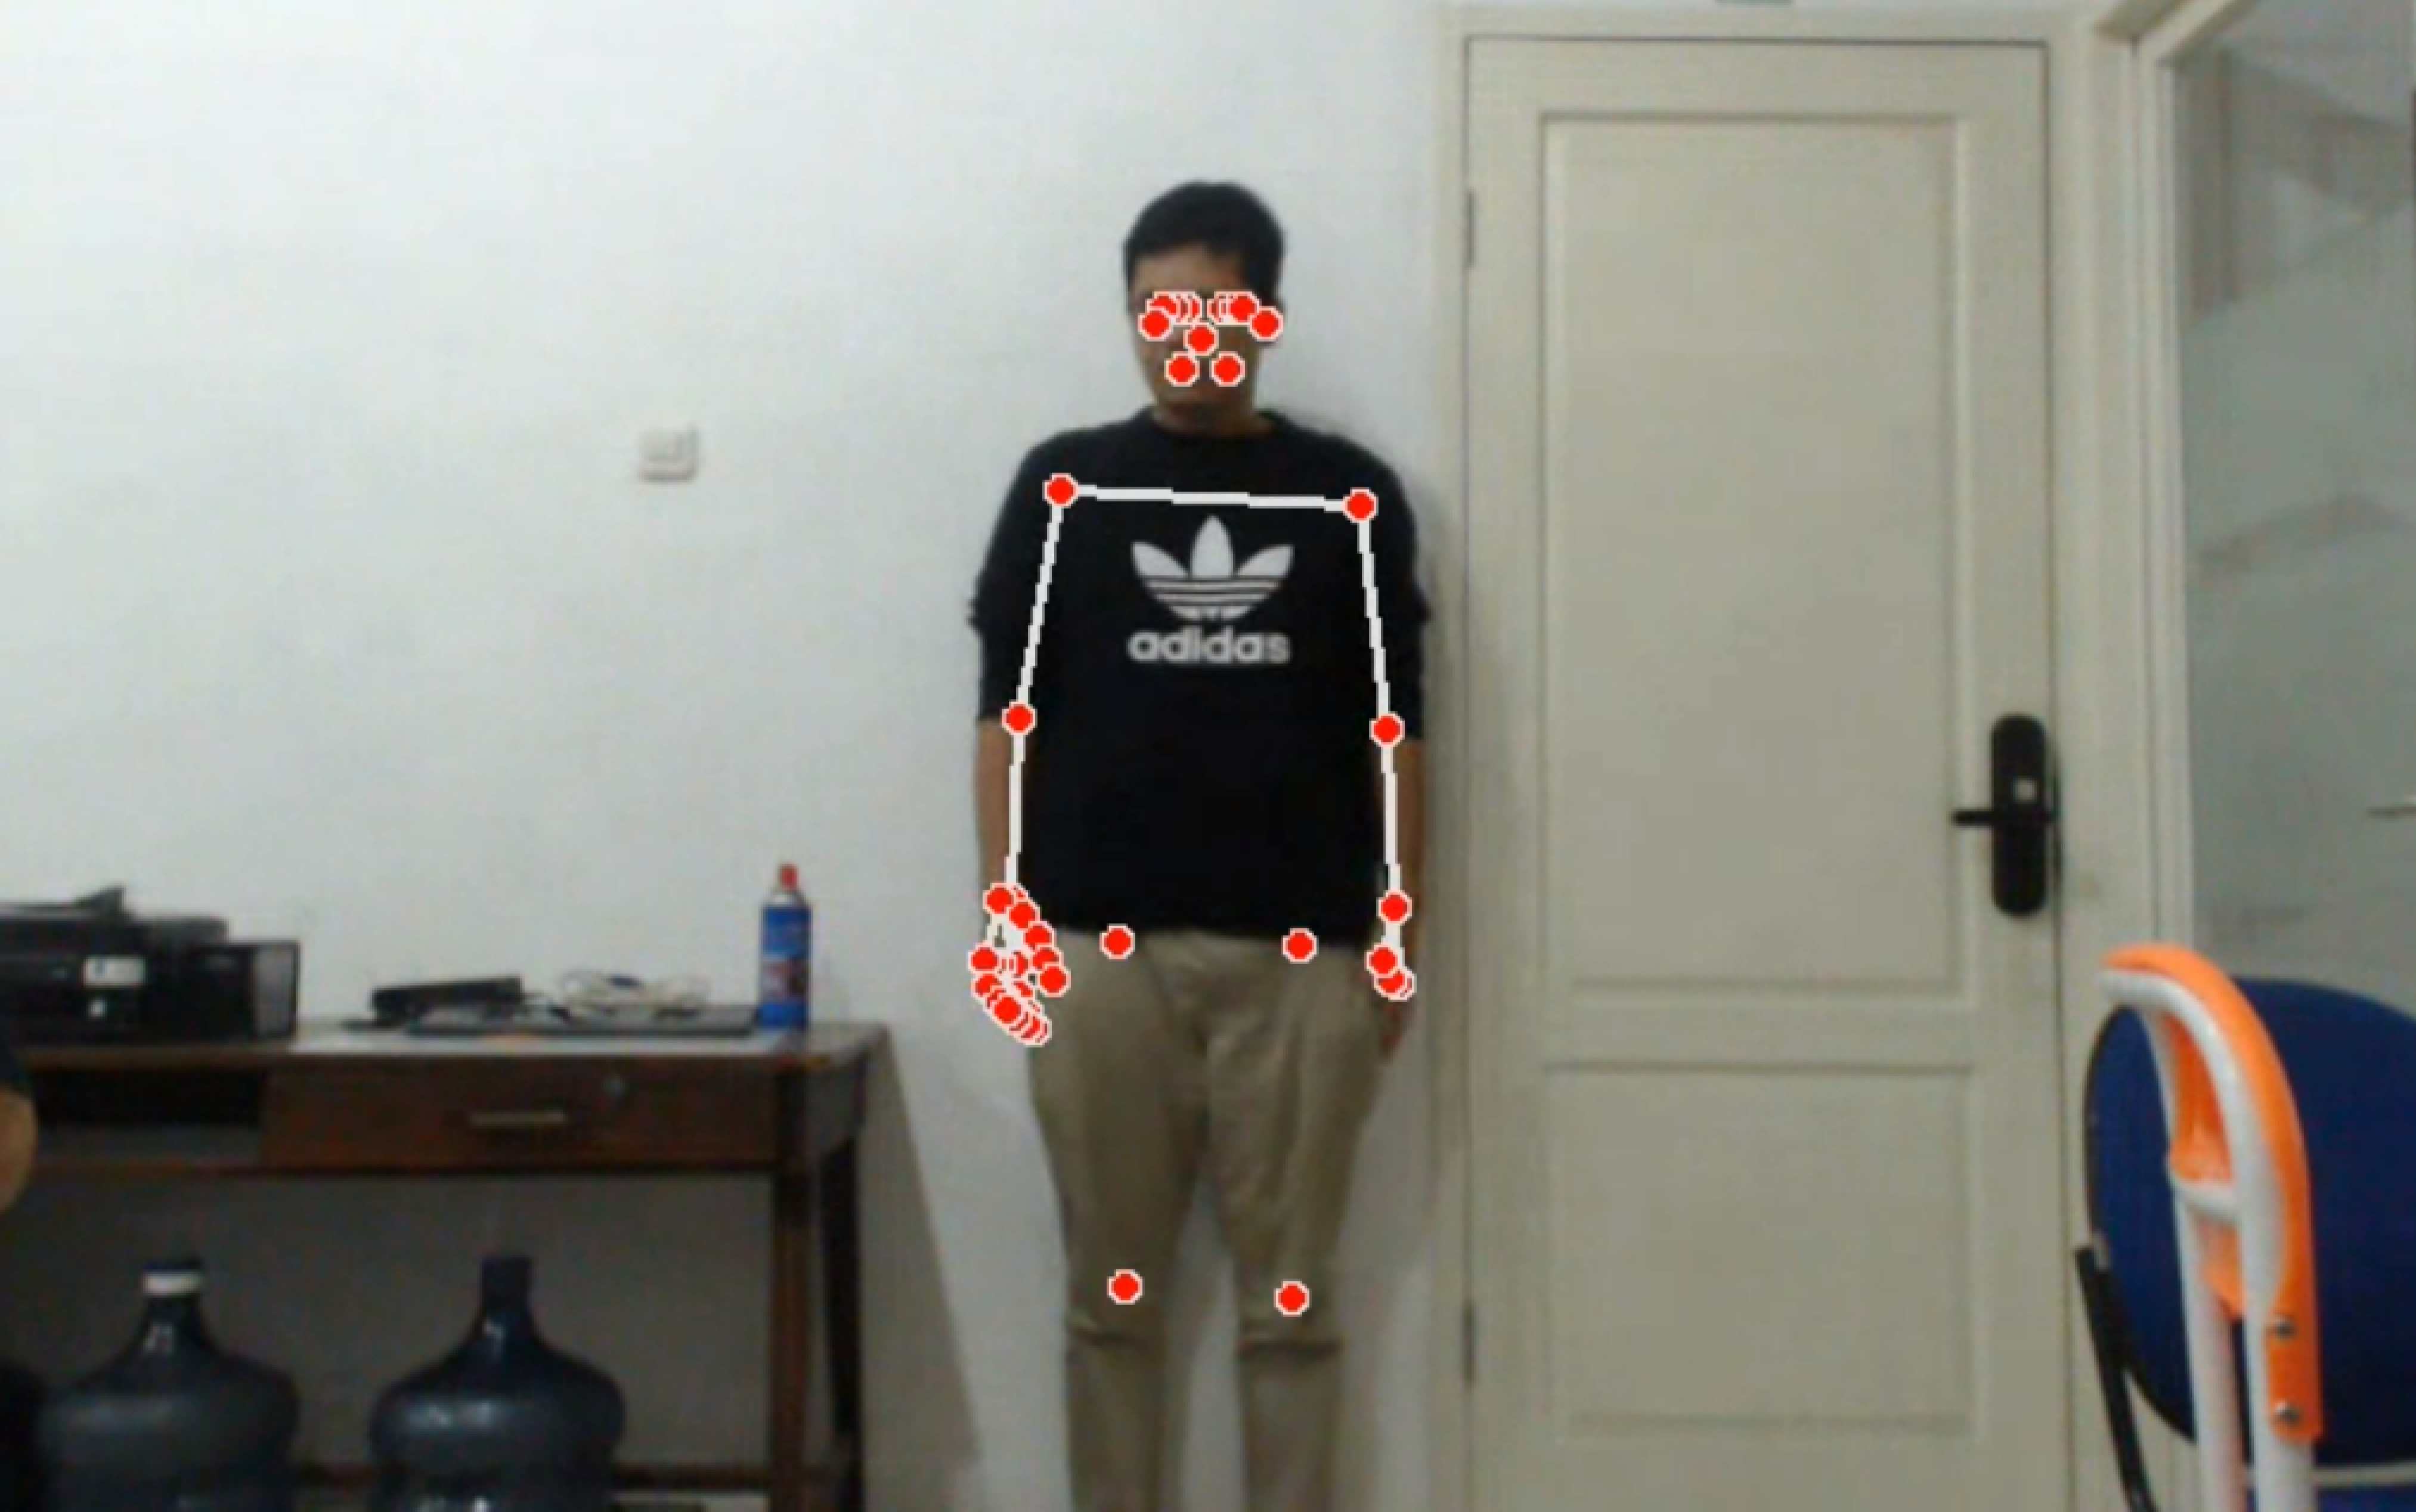
\includegraphics[scale=0.3]{gambar/bab4-evan.png}                 \\
  \hline
\end{longtable}

Pada pengujian dengan menggunakan subjek yang berbeda ini dilakukan untuk memahami bagaimana performa model pada pengguna selain darii penulis. Hal ini dilakukan demi melihat apakah model berhasil beradaptasi terhadap data yang bukan merupakan dataset yang digunakan dalam \emph{training} sehingga kedepannya dapat digunakan oleh kalangan luas. Adapun subjek yang akan diujikan berjumlah 2, yaitu 1 perempuan dan 1 laki - laki. Adapun gambaran subjek yang akan diujikan dapat dilihat pada tabel \ref{tb:kondisisubjek}. 

Model penerjemah bahasa Indonesia (BISINDO) yang akan digunakan pada pengujian ini adalah model pada bagian \ref{sec:analisismodel3} karena merupakan model yang menghasilkan klasifikasi yang terbaik jika dibandingkan dengan model lainnya. Untuk setiap intensitas cahaya akan dilakukan pengujian sebanyak tiga kali dengan jarak terhadap kamera sebesar 300 cm dan intensitas cahaya yang berkisar pada nilai 125 lux atau kondisi ruangan terang. Pada setiap pengujian akan dicari hasil klasifikasi model, waktu yang dibutuhkan model untuk menghasilkan klasifikasi bahasa isyarat berdasarkan data koordinat yang diberikan(\emph{processing time}), dan waktu total yang dibutuhkan dalam menghasilkan klasifikasi bahasa isyarat (\emph{complete time}).  

\subsection{Pengujian Subjek Perempuan}
\label{sec:analisisperempuan}

\begin{longtable}{|c|c|c|c|}
  \caption{Pengujian Pertama Model di Subjek Berbeda Perempuan}
  \label{tb:prediksiperempuan1}                                   \\
  \hline
  \rowcolor[HTML]{C0C0C0}
  \textbf{Kosakata} & \textbf{Klasifikasi Model} & \textbf{\emph{Processing Time}} & \textbf{\emph{Complete Time}}\\
  \hline
  Maaf              & \textcolor{red}{Tolong}       & 0.09316182136535645 detik                           & 3.208651542663574 detik                                \\
  Tolong            & Tolong                        & 0.0934598445892334 detik                            & 2.874863147735596 detik                                \\
  Nama              & Nama                          & 0.09218382835388184 detik                           & 3.2549500465393066 detik                                 \\
  Saya              & Saya                          & 0.09529590606689453 detik                           & 3.128707408905029 detik                                \\
  Siapa              & Siapa                        & 0.09517526626586914 detik                           & 2.9302382469177246 detik                                 \\
  Rumah             & \textcolor{red}{Delete}       & 0.1019589900970459 detik                            & 3.019108772277832 detik                                \\
  Delete            & Delete                        & 0.10392284393310547 detik                           & 3.0571460723876953 detik                                 \\
  Standby           & Standby                       & 0.09529590606689453 detik                           & 1.4797425270080564 detik                                 \\
  Translate         & Translate                     & 0.0931706428527832 detik                            & 2.943220138549805 detik                                \\
  \hline
\end{longtable}

\begin{longtable}{|c|c|c|c|}
  \caption{Pengujian Kedua Model di Subjek Berbeda Perempuan}
  \label{tb:prediksiperempuan2}                                   \\
  \hline
  \rowcolor[HTML]{C0C0C0}
  \textbf{Kosakata} & \textbf{Klasifikasi Model} & \textbf{\emph{Processing Time}} & \textbf{\emph{Complete Time}}\\
  \hline
  Maaf              & Maaf                         & 0.09658217430114746 detik                           & 3.1087589263916016 detik                                  \\
  Tolong            & Tolong                       & 0.0983424186706543 detik                            & 2.8928446769714355 detik                                  \\
  Nama              & Nama                         & 0.09464740753173828 detik                           & 2.980277538299561 detik                                 \\
  Saya              & Saya                         & 0.09416389465332031 detik                           & 2.925252914428711 detik                                 \\
  Siapa             & Siapa                        & 0.0978078842163086 detik                            & 2.927734851837158 detik                                 \\
  Rumah             & Rumah                        & 0.09566903114318848 detik                           & 3.064112663269043 detik                                 \\
  Delete            & Delete                       & 0.10792422294616699 detik                           & 3.3718514442443848 detik                                  \\
  Standby           & Standby                      & 0.09643745422363281 detik                           & 1.5385866165161133 detik                                  \\
  Translate         & Translate                    & 0.10363197326660156 detik                           & 2.9689049720764165 detik                                  \\
  \hline
\end{longtable}

\newpage
\begin{longtable}{|c|c|c|c|}
  \caption{Pengujian Ketiga Model di Subjek Berbeda Perempuan}
  \label{tb:prediksiperempuan3}                                   \\
  \hline
  \rowcolor[HTML]{C0C0C0}
  \textbf{Kosakata} & \textbf{Klasifikasi Model} & \textbf{\emph{Processing Time}} & \textbf{\emph{Complete Time}}\\
  \hline
  Maaf              & Maaf                        & 0.09667658805847168 detik                           & 3.103616237640381 detik                                 \\
  Tolong            & Tolong                      & 0.09738278388977051 detik                           & 3.0499148368835454 detik                                  \\
  Nama              & Nama                        & 0.09640955924987793 detik                           & 2.927877902984619 detik                                 \\
  Saya              & Saya                        & 0.0947885513305664 detik                            & 1.4657378196716309 detik                                  \\
  Siapa             & Siapa                       & 0.09821367263793945 detik                           & 3.0816650390625 detik                               \\
  Rumah             & Rumah                       & 0.09819889068603516 detik                           & 2.870771884918213 detik                                 \\
  Delete            & Delete                      & 0.11416792869567871 detik                           & 3.0212616920471187 detik                                  \\
  Standby           & Standby                     & 0.09473133087158203 detik                           & 1.5490007400512695 detik                                  \\
  Translate         & Translate                   & 0.09832525253295898 detik                           & 3.1276202201843266 detik                                  \\
  \hline
\end{longtable}

Berdasarkan tiga pengujian yang telah dilakukan, didapatkan bahwa hampir keseluruhan klasifikasi model yang sesuai dengan \emph{class} kosakata. Namun, terdapat beberapa kesalahan model dalam melakukan klasifikasi. Dapat dilihat pada tabel \ref{tb:prediksiperempuan1} untuk isyarat kosakata "Maaf" diklasifikasikan sebagai "Tolong". Hal ini dapat disebabkan oleh kesalahan pola gerakan isyarat yang digunakan, dimana kurang ditekankannya keunikan atau \emph{feature} dari masing - masing gerakan bahasa isyarat.  Secara garis besar, hasil pengujian ini menunjukkan bahwa model dengan mudah dapat mengklasifikasikan bahasa isyarat yang diperagakan oleh pengguna dengan jenis kelamin perempuan dengan akurasi sebesar 92.5\%. 

Apabila dilihat berdasarkan waktu pemrosesan, rata - rata waktu yang dibutuhkan model untuk menghasilkan klasifikasi bahasa isyarat (\emph{processing time}) adalah 0.098 detik dan rata - rata waktu yang dibutuhkan dalam menghasilkan klasifikasi bahasa isyarat (\emph{complete time}) adalah 2.810 detik. Hal ini menunjukkan bahwa pada subjek perempuan yang berbeda dengan penulis tidak mempengaruhi nilai \emph{processing time} dan \emph{complete time}. Juga data ini semakin menguatkan bahwa model telah dapat beradaptasi dengan subjek yang berbeda dengan penulis.  

\subsection{Pengujian Subjek Laki - Laki}
\label{sec:analisislaki}

\begin{longtable}{|c|c|c|c|}
  \caption{Pengujian Pertama Model di Subjek Berbeda Laki - Laki}
  \label{tb:prediksilaki1}                                   \\
  \hline
  \rowcolor[HTML]{C0C0C0}
  \textbf{Kosakata} & \textbf{Klasifikasi Model} & \textbf{\emph{Processing Time}} & \textbf{\emph{Complete Time}}\\
  \hline
  Maaf              & \textcolor{red}{Tolong}        & 0.10172176361083984 detik                           & 3.0670595169067383 detik                                  \\
  Tolong            & Tolong                         & 0.09742546081542969 detik                           & 3.017871379852295 detik                                 \\
  Nama              & Nama                           & 0.09616494178771973 detik                           & 3.0398440361022954 detik                                  \\
  Saya              & Saya                           & 0.10310554504394531 detik                           & 1.4680695533752441 detik                                  \\
  Siapa             & Siapa                          & 0.10661101341247559 detik                           & 2.922499179840088 detik                                 \\
  Rumah             & \textcolor{red}{Delete}        & 0.08926630020141602 detik                           & 2.829294204711914 detik                                 \\
  Delete            & Delete                         & 0.09601879119873047 detik                           & 3.159763813018799 detik                                 \\
  Standby           & Standby                        & 0.09913754463195801 detik                           & 1.5385866165161133 detik                                  \\
  Translate         & Translate                      & 0.10099458694458008 detik                           & 2.9112768173217773 detik                                  \\
  \hline
\end{longtable}

\newpage
\begin{longtable}{|c|c|c|c|}
  \caption{Pengujian Kedua Model di Subjek Berbeda Laki - Laki}
  \label{tb:prediksilaki2}                                   \\
  \hline
  \rowcolor[HTML]{C0C0C0}
  \textbf{Kosakata} & \textbf{Klasifikasi Model} & \textbf{\emph{Processing Time}} & \textbf{\emph{Complete Time}}\\
  \hline
  Maaf              & Maaf                         & 0.10624909400939941 detik                           & 2.9753994941711426 detik                                  \\
  Tolong            & Tolong                       & 0.09604954719543457 detik                           & 2.9878664016723637 detik                                  \\
  Nama              & Nama                         & 0.09938287734985352 detik                           & 2.855043411254883 detik                                 \\
  Saya              & Saya                         & 0.09951472282409668 detik                           & 1.5473628044128418 detik                                  \\
  Siapa             & Siapa                        & 0.08862924575805664 detik                           & 2.881293296813965 detik                                 \\
  Rumah             & Rumah                        & 0.08926630020141602 detik                           & 2.879476547241211 detik                                 \\
  Delete            & Delete                       & 0.09708309173583984 detik                           & 3.097364902496338 detik                                 \\
  Standby           & Standby                      & 0.10267424583435059 detik                           & 1.5490007400512695 detik                                  \\
  Translate         & Translate                    & 0.10302090644836426 detik                           & 3.1186795234680176 detik                                  \\
  \hline
\end{longtable}

\begin{longtable}{|c|c|c|c|}
  \caption{Pengujian Ketiga Model di Subjek Berbeda Laki - Laki}
  \label{tb:prediksilaki3}                                   \\
  \hline
  \rowcolor[HTML]{C0C0C0}
  \textbf{Kosakata} & \textbf{Klasifikasi Model} & \textbf{\emph{Processing Time}} & \textbf{\emph{Complete Time}}\\
  \hline
  Maaf              & Maaf                          & 0.09524083137512207 detik                           & 3.0119776725769043 detik                                  \\
  Tolong            & Tolong                        & 0.10116004943847656 detik                           & 3.0259251594543457 detik                                 \\
  Nama              & Nama                          & 0.10364699363708496 detik                           & 2.9966139793395996 detik                                 \\
  Saya              & Saya                          & 0.0972299575805664 detik                            & 1.4724183082580566 detik                                 \\
  Siapa             & Siapa                         & 0.09995222091674805 detik                           & 2.967231273651123 detik                                \\
  Rumah             & Rumah                         & 0.08926630020143602 detik                           & 2.9637622833251953 detik                                 \\
  Delete            & Delete                        & 0.09006118774414062 detik                           & 2.9045462608337402 detik                                 \\
  Standby           & Standby                       & 0.10000467300415039 detik                           & 2.028508186340332 detik                                \\
  Translate         & Translate                     & 0.10082817077636719 detik                           & 3.1959056854248047 detik                                 \\
  \hline
\end{longtable}

Berdasarkan tiga pengujian yang telah dilakukan, didapatkan bahwa hampir keseluruhan klasifikasi model yang sesuai dengan \emph{class} kosakata. Namun, terdapat beberapa kesalahan model dalam melakukan klasifikasi. Dapat dilihat pada tabel \ref{tb:prediksilaki1} untuk kosakata isyarat "Maaf" diklasifikasikan sebagai "Tolong". Hal ini dapat disebabkan oleh kesalahan pola gerakan isyarat yang digunakan, dimana kurang ditekankannya keunikan atau \emph{feature} dari masing - masing gerakan bahasa isyarat.  Secara garis besar, hasil pengujian ini menunjukkan bahwa model dengan mudah dapat mengklasifikasikan bahasa isyarat yang diperagakan oleh pengguna dengan jenis kelamin perempuan dengan akurasi sebesar 92.5\%. 

Apabila dilihat berdasarkan waktu pemrosesan, rata - rata waktu yang dibutuhkan model untuk menghasilkan klasifikasi bahasa isyarat (\emph{processing time}) adalah 0.098 detik dan rata - rata waktu yang dibutuhkan dalam menghasilkan klasifikasi bahasa isyarat (\emph{complete time}) adalah 2.682 detik. Hal ini menunjukkan bahwa pada subjek yang berbeda dengan penulis tidak mempengaruhi \emph{processing time} dan \emph{complete time}. Data ini juga menunjukkan bahwa proses normalisasi yang dilakukan telah berhasil dan memudahkan model untuk mengklasifikasikan gerakan bahasa isyarat secara \emph{general} atau menyeluruh.  

\newpage
\subsection{Rangkuman Pengujian Subjek Berbeda}
\label{sec:analisissubjekberbeda}

\begin{longtable}{|c|c|c|c|}
  \caption{Rangkuman Pengujian Subjek Berbeda}
  \label{tb:evaluasiSubjek}                                   \\
  \hline
  \rowcolor[HTML]{C0C0C0}
  \textbf{Subjek} & \textbf{Akurasi} & \emph{\textbf{Avg. Processing Time}} & \emph{\textbf{Avg. Complete Time}} \\
  \hline
  Perempuan & 0.93   & 0.0988 detik & 2.6636 detik \\
  Laki - Laki & 0.93 & 0.0973 detik & 2.8191 detik \\
  \hline
\end{longtable}

Secara keseluruhan, dapat dilihat bahwa model dapat bekerja untuk melakukan klasifikasi berdasarkan gerakan isyarat dari subjek yang berbeda dengan penulis. Normalisasi data yang dilakukan telah berhasil menggeneralisasi data sehingga model dapat menghasilkan klasifikasi yang baik meskipun berasal dari subjek yang berbeda dari penulis. Hal ini dibuktikan dengan akurasi pada subjek laki - laki dan perempuan bernilai 0.93 atau 93\%. Adapun nilai dari \emph{average processing time} dan \emph{average complete time} berkisar pada 0.09 detik dan 2.6 detik. Data ini tidak jauh berbeda dengan bebrapa pengujian sebelumnya yang telah dilakukan oleh penulis.

\section{Pengujian Pembentukan Kalimat dan Konversi Suara}
\label{sec:analisiskalimat}

Pada pengujian pembentukan kalimat dan konversi suara ini dilakukan untuk memahami bagaimana sistem penerjemah bahasa isyarat Indonesia (BISINDO) jika digunakan untuk membentuk kalimat dan melakukan konversi suara berdasarkan kalimat yang dibentuk. Adapun sistematika dalam pembentukan kalimat dan konversi ini mengacu dengan \emph{flowchart} yang telah dijelaskan pada sub bab \ref{sec:metodologisistemkontrol}. Kombinasi kata untuk membentuk kalimat pada sistem ini dapat dilihat pada tabel \ref{tb:kalimatpengujian}. Perlu diperhatikan bahwa untuk mendeteksi kosakata dan mengontrol sistem (\emph{translate} dan \emph{delete}) memerlukan pengguna untuk berada di keadaan \emph{standby} terlebih dahulu. Pembentukan kalimat dan konveri suara pada pengujian ini dilakukan secara sekuensial dengan memastikan bahwa setiap kosakata benar terklasifikasi. Kemudian, kalimat akan diterjemahkan dengan melakukan gerakan isyarat kontrol "\emph{translate}" dan diakhiri dengan melakukan gerakan isyarat kontrol "\emph{delete}" untuk memastikan bahwa kosakata terakhir berhasil dihapus. Pengulangan bahasa isyarat dilakukan maksimal sebanyak tiga kali.

\begin{longtable}{|c|c|}
  \caption{Kalimat Pengujian}
  \label{tb:kalimatpengujian}                                   \\
  \hline
  \rowcolor[HTML]{C0C0C0}
  \textbf{Kombinasi Kosakata} & \textbf{Kalimat Akhir}  \\
  \hline
  "Maaf" + "Siapa" + "Nama"            &  "Maaf siapa nama kamu?"               \\

  "Maaf" + "Tolong "+ "Saya"            & "Maaf tolong bantu saya"                 \\
  
  "Maaf" + "Rumah" + "Siapa"            & "Maaf ini rumah siapa?"                 \\

  "Rumah" + "Saya"            & "Ini rumah saya"                 \\

  "Rumah" + "Siapa"            & "Ini rumah siapa"                 \\

  "Siapa" + "Nama"            & "Siapa nama kamu?"                 \\

  "Tolong" + "Saya"            & "Tolong bantu saya"                 \\
  \hline
\end{longtable}

Model penerjemah bahasa Indonesia (BISINDO) yang akan digunakan pada pengujian ini adalah model pada bagian \ref{sec:analisismodel3} karena merupakan model yang menghasilkan klasifikasi yang terbaik jika dibandingkan dengan model lainnya. Untuk setiap kombinasi kalimat akan dilakukan pengujian sebanyak satu kali dengan kondisi ruangan yang memiliki intensitas cahaya yang terang (berkisar pada 125 lux) dan jarak kamera dengan pengguna bernilai 300 cm. Pada setiap kombinasi kalimat akan dicari hasil klasifikasi model, waktu yang dibutuhkan model untuk menghasilkan klasifikasi bahasa isyarat berdasarkan data koordinat yang diberikan(\emph{processing time}), dan waktu total yang dibutuhkan dalam menghasilkan klasifikasi bahasa isyarat (\emph{complete time}).  

\begin{longtable}{|c|c|c|c|}
  \caption{Pengujian Pembentukan Kalimat Pertama}
  \label{tb:prediksikombinasi1}                                   \\
  \hline
  \rowcolor[HTML]{C0C0C0}
  \textbf{Kosakata} & \textbf{Klasifikasi Model} & \textbf{\emph{Processing Time}} & \textbf{\emph{Complete Time}}\\
  \hline
  Maaf                & Maaf                          & 0.09733414649963379 detik                           & 3.103902339935303 detik                                 \\
  Siapa               & Siapa                         & 0.0981595516204834 detik                            & 2.81724214553833 detik                                \\
  Nama                & Nama                          & 0.09517359733581543 detik                           & 3.097071647644043 detik                                 \\
  Delete              & Delete                        & 0.09404182434082031 detik                           & 3.1426548957824707 detik                                  \\
  Translate           & Translate                     & 0.09448504447937012 detik                           & 2.94607400894165 detik                                \\
  \hline
\end{longtable}

\begin{longtable}{|c|c|c|c|}
  \caption{Pengujian Pembentukan Kalimat Kedua}
  \label{tb:prediksikombinasi2}                                   \\
  \hline
  \rowcolor[HTML]{C0C0C0}
  \textbf{Kosakata} & \textbf{Klasifikasi Model} & \textbf{\emph{Processing Time}} & \textbf{\emph{Complete Time}}\\
  \hline
  Maaf              & Maaf                          & 0.10064482688903809 detik                           & 2.822299003601074 detik                                 \\
  Tolong            & Tolong                        & 0.09766435623168945 detik                           & 2.844550609588623 detik                                 \\
  Saya              & Nama                          & 0.09680485725402832 detik                           & 2.9134011268615723 detik                                  \\
  Delete              & Delete                      & 0.09553837776184082 detik                           & 3.1421828269958496 detik                                  \\
  Translate              & Translate                & 0.09472537040710449 detik                           & 2.8847408294677734 detik                                  \\
  \hline
\end{longtable}

\begin{longtable}{|c|c|c|c|}
  \caption{Pengujian Pembentukan Kalimat Ketiga}
  \label{tb:prediksikombinasi3}                                   \\
  \hline
  \rowcolor[HTML]{C0C0C0}
  \textbf{Kosakata} & \textbf{Klasifikasi Model} & \textbf{\emph{Processing Time}} & \textbf{\emph{Complete Time}}\\
  \hline
  Maaf              & Maaf                          & 0.10550785064697266 detik                           & 2.969491481781006 detik                                 \\
  Rumah            & Tolong                         & 0.0971059799194336  detik                           & 2.9895544052124023 detik                                  \\
  Siapa              & Nama                         & 0.10715579986572266 detik                           & 2.9179072380065922 detik                                  \\
  Delete              & Delete                      & 0.0979464054107666  detik                           & 2.9804134368896484 detik                                  \\
  Translate              & Translate                & 0.10163474082946777 detik                           & 2.958190441131592 detik                                 \\
  \hline
\end{longtable}

\begin{longtable}{|c|c|c|c|}
  \caption{Pengujian Pembentukan Kalimat Keempat}
  \label{tb:prediksikombinasi4}                                   \\
  \hline
  \rowcolor[HTML]{C0C0C0}
  \textbf{Kosakata} & \textbf{Klasifikasi Model} & \textbf{\emph{Processing Time}} & \textbf{\emph{Complete Time}}\\
  \hline
  Rumah               & \textcolor{red}{Delete}       & 0.09740185737609863 detik                           & 3.042304515838623 detik                                 \\
  Saya                & Saya                          & 0.0987851619720459 detik                            & 1.4961934089660645 detik                                  \\
  Delete              & Delete                        & 0.09497356414794922 detik                           & 2.9061841964721684 detik                                  \\
  Translate           & Translate                     & 0.10316205024719238 detik                           & 2.943763732910156 detik                                 \\
  \hline
\end{longtable}

\newpage
\begin{longtable}{|c|c|c|c|}
  \caption{Pengujian Pembentukan Kalimat Kelima}
  \label{tb:prediksikombinasi5}                                   \\
  \hline
  \rowcolor[HTML]{C0C0C0}
  \textbf{Kosakata} & \textbf{Klasifikasi Model} & \textbf{\emph{Processing Time}} & \textbf{\emph{Processing Time}}\\
  \hline
  Rumah               & Rumah                         & 0.09344840049743652 detik                           & 1.5613818168640137 detik                                  \\
  Siapa               & Siapa                         & 0.09488558769226074 detik                           & 1.4586281776428223 detik                                  \\
  Delete              & Delete                        & 0.09873461723327637 detik                           & 3.033885955810547  detik                                 \\
  Translate           & Translate                     & 0.1056978702545166 detik                            & 2.9063844680786133 detik                                  \\
  \hline
\end{longtable}

\begin{longtable}{|c|c|c|c|}
  \caption{Pengujian Pembentukan Kalimat Keenam}
  \label{tb:prediksikombinasi6}                                   \\
  \hline
  \rowcolor[HTML]{C0C0C0}
  \textbf{Kosakata} & \textbf{Klasifikasi Model} & \textbf{\emph{Processing Time}} & \textbf{\emph{Complete Time}}\\
  \hline
  Siapa               & Siapa                         & 0.10315442085266113 detik                           & 3.042304515838623 detik                                 \\
  Nama                & Nama                          & 0.0998544692993164  detik                           & 1.4961934089660645 detik                                  \\
  Delete              & Delete                        & 0.09890484809875488 detik                           & 2.9061841964721684 detik                                  \\
  Translate           & Translate                     & 0.10316205024719238 detik                           & 2.943763732910156 detik                                 \\
  \hline
\end{longtable}

\begin{longtable}{|c|c|c|c|}
  \caption{Pengujian Pembentukan Kalimat Ketujuh}
  \label{tb:prediksikombinasi7}                                   \\
  \hline
  \rowcolor[HTML]{C0C0C0}
  \textbf{Kosakata} & \textbf{Klasifikasi Model} & \textbf{\emph{Processing Time}} & \textbf{\emph{Complete Time}}\\
  \hline
  Tolong              & Tolong                        & 0.10103940963745117 detik                          & 3.0083799362182617 detik                                  \\
  Saya                & Saya                          & 0.10042452812194824 detik                          & 2.944457530975342 detik                                 \\
  Delete              & Delete                        & 0.0952444076538086 detik                           & 3.03605318069458  detik                                \\
  Translate           & Translate                     & 0.10302400588989258 detik                          & 3.0155038833618164 detik                                  \\
  \hline
\end{longtable}

% \begin{longtable}{|c|c|}
%   \caption{Waktu \emph{Translate} Kombinasi Kalimat}
%   \label{tb:waktutranslate}                                   \\
%   \hline
%   \rowcolor[HTML]{C0C0C0}
%   \textbf{Kalimat} & \textbf{Waktu Penyuaraan Kalimat}\\
%   \hline
%   Maaf siapa nama kamu?              & 1.9165489673614502                               \\
%   Maaf tolong bantu saya            & 1.824713945388794                            \\
%   Maaf ini rumah siapa?              & 1.9595482349395752                         \\
%   Ini rumah saya              & 1.5204029083251953                             \\
%   Ini rumah siapa?              & 1.605020523071289                             \\
%   Siapa nama kamu?              & 1.606485366821289                             \\
%   Tolong bantu saya              & 1.5231249332427979                             \\
%   \hline
% \end{longtable}

Untuk kalimat yang terdiri dari kombinasi tiga kosakata, yaitu kalimat pertama, kalimat kedua, dan kalimat ketiga telah berhasil dibentuk. Hal ini dapat dilihat dari untuk kombinasi kosakata pembentuk kalimat tersebut telah berhasil diklasifikasikan dengan akurasi sebesar 100\% (dapat dilihat pada tabel \ref{tb:prediksikombinasi1}, tabel \ref{tb:prediksikombinasi2}, dan tabel \ref{tb:prediksikombinasi3}). Pada kalimat pertama, rata - rata \emph{processing time} bernilai 0.096 detik dan \emph{complete time} bernilai 3.021 detik. Pada kalimat kedua, rata - rata \emph{processing time} bernilai 0.097 detik dan \emph{complete time} bernilai 2.921 detik. Pada kalimat ketiga, rata - rata \emph{processing time} bernilai 0.102 detik dan \emph{complete time} bernilai 2.963 detik. Dapat dilihat bahwa meskipun gerakan bahasa isyarat dilakukan secara sekuensial, tetap dapat menghasilkan klasifikasi akurasi yang baik.

Untuk kalimat yang terdiri dari kombinasi dua kosakata, yaitu kalimat kelima, keenam, dan ketujuh telah berhasil dibentuk. Hal ini dapat dilihat dari kombinasi kosakata pembentuk kalimat tersebut telah berhasil diklasifikasikan dengan akurasi sebesar 93.75\% (dapat dilihat pada tabel \ref{tb:prediksikombinasi5}, \ref{tb:prediksikombinasi6}, \ref{tb:prediksikombinasi7}). Pada kalimat kelima, rata - rata \emph{processing time} bernilai 0.098 detik dan \emph{complete time} bernilai 2.240 detik. Pada kalimat keenam, rata - rata \emph{processing time} bernilai 0.100 detik dan \emph{complete time} bernilai 2.199 detik.Pada kalimat ketujuh, rata - rata \emph{processing time} bernilai 0.100 detik dan \emph{complete time} bernilai 3.001 detik. Dapat dilihat bahwa untuk \emph{complete time} relatif lebih cepat pada kalimat dengan kombinasi tiga kosakata jika dibandingkan dengan kalimat dengan kombinasi dua kosakata.

Namun, pada kalimat keempat ("Ini rumah saya") terdapat kosakata yang salah sehingga menyebabkan gagalnya terbentuk kalimat tersebut dalam pengujian yang dilakukan secara sekue\\nsial. Isyarat kosakata "Rumah" diklasifikasikan sebagai "Delete". Hal ini dapat disebabkan oleh adanya kemiripan gerakan antara kedua kosakata tersebut. rata - rata \emph{processing time} bernilai 0.099 detik dan \emph{complete time} bernilai 2.597 detik.

\subsection{Rangkuman Pengujian Pembentukan Kalimat dan Konveri Suara}
\label{sec:analisikalimatsuara}

\begin{longtable}{|c|c|c|c|}
  \caption{Rangkuman Pengujian Pembentukan Kalimat dan Konveri Suara}
  \label{tb:evaluasiKalimatdanSuara}                                   \\
  \hline
  \rowcolor[HTML]{C0C0C0}
  \textbf{Kosakata} & \textbf{Akurasi} & \emph{\textbf{Avg. Processing Time}} & \emph{\textbf{Avg. Complete Time}} \\
  \hline
  2 kosakata & 1.00 & 0.0993 detik & 2.8303 detik \\
  3 kosakata & 0.93 & 0.0981 detik & 2.0513 detik \\
  \hline
\end{longtable}

Secara keseluruhan, dapat dilihat bahwa sistem penerjemah dapat melakukan klasifikasi dengan baik dalam menerjemahkan gerakan isyarat yang dilakukan secara sekuensial. Hal ini tidak berdampak secara signifikan terhadap \emph{average processing time} dan \emph{average complete time}. Akurasi klasifikasi masih sangat baik, dimana pada kalimat dengan 2 kosakata bernilai 1.00 atau 100\% dan 3 kosakata bernilai 0.93 atau 93\%. Pada kalimat dengan 3 kosakata, hanya 1 kalimat yang tidak berhasil untuk dibentuk, yaitu kalimat "Ini rumah saya". Library gtts (Google Text-To-Speech) telah dapat berfungsi dengan baik untuk menkonversi data teks dalam bentuk \emph{string} ke dalam suara sesuai dengan kalimat yang ditandai dengan gerakan isyarat \emph{translate} yang berhasil dideteksi pada setiap percobaan. Adapun secara keseluruhan, tingkat keberhasilan sistem penerjemah dalam membentuk kalimat adalah sebesar 85.7\%.

% Untuk kalimat yang terdiri dari kombinasi tiga kosakata, pada kombinasi kalimat pertama didapat bahwa keseluruhan kosakata bahasa isyarat untuk kalimat "Maaf siapa nama kamu?" telah berhasil dibentuk. Hal ini dapat dilihat untuk seluruh kombinasi kosakata yang telah berhasil diklasifikasikan dengan akurasi sebesar 100\%. Untuk rata - rata \emph{processing time} dan \emph{complete time} adalah 0.096 detik  dan 3.021 detik. Pada kombinasi kalimat kedua, keseluruhan kosakata bahasa isyarat untuk kalimat "Maaf tolong bantu saya?" telah berhasil dibentuk. Hal ini dapat dilihat untuk seluruh kombinasi kosakata yang telah berhasil diklasifikasikan dengan akurasi sebesar 100\%. Untuk rata - rata \emph{processing time} dan \emph{complete time} adalah 0.097 detik  dan 2.921 detik. Pada kombinasi kalimat ketiga, keseluruhan kosakata bahasa isyarat untuk kalimat "Maaf ini rumah siapa?" telah berhasil dibentuk. Hal ini dapat dilihat untuk seluruh kombinasi kosakata yang telah berhasil diklasifikasikan dengan akurasi sebesar 100\%. Untuk rata - rata \emph{processing time} dan \emph{complete time} adalah 0.102 detik  dan 2.963 detik.

% Untuk kalimat yang terdiri dari kombinasi dua kosakata, pada kombinasi kalimat keempat didapat bahwa keseluruhan kosakata bahasa isyarat untuk kalimat "Ini rumah saya" tidak berhasil dibentuk. Hal ini disebabkan oleh kosakata "Rumah" diklasifikasikan sebagai "Delete". Untuk rata - rata \emph{processing time} dan \emph{complete time} adalah 0.096 detik dan 3.021 detik. Pada kombinasi kalimat keenam, keseluruhan bahasa isyarat untuk kalimat "Maaf tolong bantu saya"  telah berhasil dibentuk. Hal ini dapat dilihat untuk seluruh kombinasi kosakata telah berhasil diklasifikasikan dengan akurasi sebesar 100\%.  Untuk rata - rata \emph{processing time} dan \emph{complete time} adalah 0.098 detik  dan 2.240 detik.

% \section{Pengujian Performa NUC}
% \label{sec:analisisnuc}
% \section{Evaluasi Pengujian}
% \label{sec:analisispengujian}

% Dari pengujian yang \lipsum[1]

% % Contoh pembuatan tabel


% \lipsum[2-4]
